% !TeX root = ../../Book1.tex
% 纲要标题：## 第11章　光滑流形、切丛与局部标准形
% 纲要位置：几何学计划纲要.md，第 533 行。
% 正文状态：初稿；尚未正式审核。

% 纲要内容开始
% 
% > 本章目标与证明范围：流形路线从本章独立进入。按“坐标相容—切映射—秩条件—局部标准形—子流形”的顺序证明，不先使用尚未定义的切丛；必要多元微分定理就地重建。
% 
% 纲要内容结束

\chapter{光滑流形、切丛与局部标准形}
\label{g1:ch:11}
\BookChapterNumber{g1:ch:11}

\begin{chapterabstract}
	流形上的微分计算由光滑换坐标相互联系，像上的拓扑则决定局部参数怎样组成整体。本章从光滑相容的图册构造球面、射影空间与带边界流形，以局部函数芽的导子定义切空间，并证明内点处与曲线速度的等价，建立切丛、余切空间和微分的链式法则。随后用压缩估计完整证明定量逆函数定理，推导参数隐函数定理与常秩定理，得到浸入、淹没和正则水平集的局部标准形。最后区分单射浸入与嵌入，证明限制映射的光滑性与固有嵌入判据，并明确边界版本所需的附加条件。
\end{chapterabstract}

\begin{learninggoals}
	\begin{itemize}
		\item 用明确的坐标图、换坐标和拓扑条件构造光滑流形，区分同胚、光滑双射与微分同胚。
		\item 从导子恢复切空间的坐标基，计算微分与余切拉回，并说明边界处完整切空间与可实现曲线速度的区别。
		\item 由导数估计构造局部逆，给出逆映射的正则性证明，并在有参数的方程中明确存在唯一性的局部范围。
		\item 用常秩坐标化简光滑映射，辨认浸入、淹没与正则水平集，计算水平集的切空间。
		\item 检查像空间的拓扑，判断单射浸入何时是嵌入；在带边界问题中分别核对微分秩与边界相交条件。
	\end{itemize}
\end{learninggoals}

一个圆周可以由方程 \(x^2+y^2=1\) 描述，也可以在小段上用角度参数化。第一种写法把它放在平面里，第二种写法只需一个实变量。若只关心圆周上的光滑函数和运动速度，究竟哪些量依赖平面，哪些量依赖角度的选择，哪些量属于圆周本身？同样的问题出现在球面、射影空间和更高维约束集合上。光滑流形把“每一小块可以使用 Euclid 微积分”组织成一个与坐标选择相容的整体结构。

\ProseParagraphBreak

光滑映射、可逆微分与像上的拓扑描述着不同的性质。映射 \(t\mapsto t^3\) 光滑且双射，逆却在零点不可微；一条参数曲线可以处处有非零速度、没有重复经过同一点，而其像的邻域仍从很远的参数处迎来另一支。要分辨这些现象，需要同时记录一阶微分、局部坐标与像上的拓扑。逆函数定理和常秩定理负责局部，嵌入的定义则保留不可由微分秩代替的整体要求。

\ProseParagraphBreak

本章可以直接开始学习，无须先通读前三编。所需基础是有限维实线性代数中的基、对偶、秩和行列式，以及多元微积分中的偏导数、全微分、链式法则和一元微积分基本定理。拓扑方面只需理解开集、连续映射、同胚、子空间与乘积；Hausdorff、第二可数和商拓扑在实际构造处作简短回顾。逆函数、隐函数和常秩三个定理在本章从 Euclid 微积分重建。没有给流形选定度量时，切向量没有预先指定的长度，余切向量也不能自动认作切向量。

\ProseParagraphBreak

可对照 Lee 第二版的第1--2章学习光滑结构与映射，第3--5章学习切空间、常秩、嵌入和子流形，第11章的 Covectors、The Differential of a Function、Pullbacks of Covector Fields 三部分学习余切与拉回\cite[第1--5章及第11章，第272--286页]{Lee2012Smooth}。这里以局部函数芽定义切空间；一般向量丛和整体构造将在\chapref{g1:ch:12}展开。带边界情形随定义和结果就近讨论，可以在第一次阅读时先理解内点证明，再对照边界处增加的条件。

% !TeX root = ../../Book1.tex
% 纲要标题：### 11.1 光滑结构与典型构造
% 纲要位置：几何学计划纲要.md，第 537 行。
% 正文状态：初稿；尚未正式审核。

% 纲要内容开始
% 
% * 图册、极大图册及光滑映射
% * 球面、射影空间、乘积与开子流形
% * 带边界流形和边界上的光滑性
% * 光滑结构与底层拓扑的区别
% 
% 纲要内容结束

\section{光滑结构与典型构造}
\label{g1:sec:1101}

在圆周的一小段上，可以用横坐标、纵坐标或适当选择的角度表示点。但横坐标在圆周的最右端不能区分邻近的上下两点，角度也不能在整条圆周上连续地取单值。流形的定义允许使用多张局部坐标图，同时要求重叠处的换坐标足够光滑。这样，在一张图中求出的导数才有可能与另一张图中的计算表达同一个对象。

\subsection{图册、极大图册及光滑映射}
\label{g1:subsec:1101:01}

先回顾本节真正需要的拓扑条件。空间是 Hausdorff 的，指任意两个不同点有不相交的开邻域；它是第二可数的，指存在可数个开集，使每个开集都能写成其中某些集合的并。前一个条件使极限不会同时落在两个不同点上，后一个条件排除无法由可数个局部坐标控制的过大空间。开子集总取给定拓扑中的开集，不能在选择坐标时另换一套拓扑。

\begin{definition}
	\label{g1:def:smooth-manifold}
	设 \(n\geq0\)，\(M\) 为 Hausdorff、第二可数拓扑空间。若 \(U\subset M\) 是开集，\(\varphi:U\to\varphi(U)\subset\mathbb R^n\) 是到欧氏开集的同胚，称 \((U,\varphi)\) 为一张\term[zuobiaotu]{坐标图}[coordinate chart]。图域覆盖 \(M\) 的坐标图族称为\term[tuce]{图册}[atlas]。两张图 \((U,\varphi)\)、\((V,\psi)\) 称为\term[guanghuaxiangrong]{光滑相容的}[smoothly compatible]，若
	\[
		\psi\circ\varphi^{-1}:\varphi(U\cap V)\longrightarrow\psi(U\cap V)
	\]
	及其逆映射都为 \(C^\infty\) 映射；交集为空时条件自动成立。两两光滑相容的图册称为\term[guanghuatuce]{光滑图册}[smooth atlas]。不能再加入新的相容坐标图的光滑图册称为\term[jidaguanghuatuce]{极大光滑图册}[maximal smooth atlas]，也称 \(M\) 的一个\term[guanghuajiegou]{光滑结构}[smooth structure]。配备这一结构的 \(M\) 称为 \(n\) 维\term[guanghualiuxing]{光滑流形}[smooth manifold]。
\end{definition}

本节先讨论无边界流形；带边界的定义在\subsecref{g1:subsec:1101:03}给出。约定 \(\mathbb R^0\) 是单点空间，因此零维流形是可数离散空间。坐标图写成 \(\varphi=(x^1,\ldots,x^n)\) 时，\(x^i\) 是定义在 \(U\) 上的实值函数，上标是坐标编号，并非幂。换坐标同时改变所有坐标函数，点 \(p\in M\) 本身不变。

\begin{proposition}
	\label{g1:prop:atlas-maximal-extension}
	设 \(\mathcal A\) 是 Hausdorff、第二可数空间 \(M\) 上的一个光滑图册。所有与 \(\mathcal A\) 中每张图相容的坐标图组成唯一包含 \(\mathcal A\) 的极大光滑图册。两个光滑图册决定同一光滑结构，当且仅当它们的并仍是光滑图册。
\end{proposition}

\begin{proof}
	记所述图族为 \(\overline{\mathcal A}\)。要证明它是图册，关键是其中新加入的两张图也相容。设 \((V,\psi)\)、\((W,\eta)\in\overline{\mathcal A}\)，在 \(p\in V\cap W\) 处选一张原图 \((U,\varphi)\in\mathcal A\) 覆盖 \(p\)。在 \(U\cap V\cap W\) 上，
	\[
		\eta\circ\psi^{-1}=(\eta\circ\varphi^{-1})\circ(\varphi\circ\psi^{-1}).
	\]
	右端两个映射都光滑，逆变换也一样。光滑性是局部性质，故两张新图在整个交叠上相容。原图已经覆盖 \(M\)，所以 \(\overline{\mathcal A}\) 是光滑图册。

	与 \(\overline{\mathcal A}\) 相容的图必与 \(\mathcal A\) 相容，因而已经包含在其中，这证明极大性。任一包含 \(\mathcal A\) 的极大图册只能由与 \(\mathcal A\) 相容的图组成，故包含于 \(\overline{\mathcal A}\)，由极大性二者相等。最后，两个图册的并若光滑，其极大扩张同时包含二者，唯一性说明两者决定同一结构；反向结论来自同一极大图册中的图两两相容。
\end{proof}

因此，给出几张足够覆盖空间的坐标图就能指定光滑结构，不必逐张列出极大图册。限制坐标图到更小开集、把欧氏坐标再作一个光滑可逆变换，都不会改变这个结构。

\ProseParagraphBreak

下面用到的欧氏微分只需要一个基本事实。映射 \(f\) 在 \(a\) 可微，意味着有线性映射 \(\mathrm{D}f(a)\) 使 \(f(a+h)=f(a)+\mathrm{D}f(a)h+o(|h|)\)。把这个式子代入 \(g\) 在 \(f(a)\) 的一阶展开，由 \(f(a+h)-f(a)=O(|h|)\) 得到
\[
	\mathrm{D}(g\circ f)(a)=\mathrm{D}g(f(a))\,\mathrm{D}f(a).
\]
这就是链式法则。各阶偏导数连续的含义也在欧氏开集上理解。逆函数定理比链式法则强得多，将在\secref{g1:sec:1103}另行证明。

\begin{definition}
	\label{g1:def:smooth-map}
	设 \(M,N\) 分别为 \(m,n\) 维光滑流形。连续映射 \(F:M\to N\) 称为\term[guanghuayingshe]{光滑映射}[smooth map]，若对每个 \(p\in M\)，可选 \(p\) 附近的图 \((U,\varphi)\) 和 \(F(p)\) 附近的图 \((V,\psi)\)，其中 \(F(U)\subset V\)，使
	\[
		\psi\circ F\circ\varphi^{-1}:\varphi(U)\longrightarrow\psi(V)
	\]
	为欧氏空间之间的 \(C^\infty\) 映射。若 \(F\) 双射，且 \(F,F^{-1}\) 都光滑，则称 \(F\) 为\term[weifentongpei]{微分同胚}[diffeomorphism]。
\end{definition}

要求 \(F(U)\subset V\) 只是为了让坐标表达有意义；连续性允许围绕任意指定的 \(p\) 缩小 \(U\) 来满足它。图中的三条箭头说明计算发生在哪里：
\[
	\begin{tikzcd}[column sep=large,row sep=large]
		U\subset M \arrow[r,"F"] \arrow[d,"\varphi"'] & V\subset N \arrow[d,"\psi"] \\
		\varphi(U)\subset\mathbb R^m \arrow[r,"\psi\circ F\circ\varphi^{-1}"'] & \psi(V)\subset\mathbb R^n.
	\end{tikzcd}
\]

\begin{proposition}
	\label{g1:prop:smooth-coordinate-independence}
	光滑映射的定义与所选相容坐标图无关。光滑映射的复合光滑，恒等映射光滑。如果非空的 \(m\) 维与 \(n\) 维光滑流形微分同胚，则 \(m=n\)。
\end{proposition}

\begin{proof}
	换成源端坐标 \(\widetilde\varphi\) 与目标坐标 \(\widetilde\psi\) 后，在共同定义的邻域中，新表达为
	\[
		\widetilde\psi\circ F\circ\widetilde\varphi^{-1}
		=(\widetilde\psi\circ\psi^{-1})\circ(\psi\circ F\circ\varphi^{-1})\circ(\varphi\circ\widetilde\varphi^{-1}).
	\]
	两侧换坐标与中间表达都光滑，故复合光滑。复合映射的结论由同样的坐标计算得到，恒等映射的坐标表达就是换坐标。

	若 \(F\) 是微分同胚，在对应点附近用坐标写 \(f\) 与 \(g=f^{-1}\)，令 \(A=\mathrm{D}f(a)\)、\(B=\mathrm{D}g(f(a))\)。由链式法则有 \(BA=I_m\)、\(AB=I_n\)，故 \(A\) 同时单射、满射，有限维线性代数给出 \(m=n\)。这里证明的是光滑可逆映射保持维数，并未把它当作一般同胚保持维数的拓扑证明。
\end{proof}

\subsection{球面、射影空间、乘积与开子流形}
\label{g1:subsec:1101:02}

给一个集合列出参数式，还没有给出流形。需要先有 Hausdorff、第二可数拓扑，再检查参数的逆是否连续、图域是否开、换坐标是否光滑。下面的构造把这些步骤逐一落实，也说明抽象定义包含了熟悉的几何对象。

\begin{example}[球面的坐标]
	\label{g1:exm:sphere-smooth-atlas}
	令 \(S^n=\{x\in\mathbb R^{n+1}:|x|=1\}\)，取欧氏子空间拓扑。对 \(i=1,\ldots,n+1\) 和 \(\varepsilon\in\{1,-1\}\)，令
	\[
		U_i^\varepsilon=\{x\in S^n:\varepsilon x_i>0\},\qquad
		\varphi_i^\varepsilon(x)=(x_1,\ldots,\widehat{x_i},\ldots,x_{n+1}),
	\]
	其中帽号表示删掉该项。像为开单位球 \(B^n\)，逆映射在第 \(i\) 位插入 \(\varepsilon\sqrt{1-|u|^2}\)。所以每张图是同胚，图域覆盖球面。换坐标只是在一个点的坐标中插入这一光滑平方根，再删去另一项，故在交叠区域光滑；逆变换同理。球面是欧氏空间的子空间，Hausdorff 性直接继承，可数欧氏开球与球面的交给出可数基。因此这些图使 \(S^n\) 成为 \(n\) 维光滑流形。

	坐标在 \(|u|=1\) 时失效，是这一张图到了边缘，球面本身没有在那里出现边界。换一张不删去零坐标的图即可继续。若 \(n\geq1\)，球面不能由一张欧氏开集坐标图覆盖：球面紧，而 \(\mathbb R^n\) 中非空开集不可能紧。后者若紧便闭，因 \(\mathbb R^n\) 连通只能等于整个 \(\mathbb R^n\)，又与其非紧性矛盾。
\end{example}

\begin{example}[实射影空间]
	\label{g1:exm:projective-smooth-atlas}
	实射影空间 \(\mathbb{RP}^n\) 的点是 \(\mathbb R^{n+1}\) 中过原点的一维线性子空间，写为 \([x_0:\cdots:x_n]\)。非零向量乘以同一非零实数表示同一点。每条直线与球面相交于一对对径点，因而给它球面商 \(S^n/(x\sim-x)\) 的拓扑。商映射 \(q:S^n\to\mathbb{RP}^n\) 是开映射，因为对球面开集 \(O\)，有 \(q^{-1}(q(O))=O\cup(-O)\)。

	令 \(U_i=\{[x]:x_i\neq0\}\)，定义
	\[
		\varphi_i([x])=(x_0/x_i,\ldots,\widehat{x_i/x_i},\ldots,x_n/x_i)\in\mathbb R^n.
	\]
	这个式子与代表向量无关。\(U_i\) 开，坐标函数连续；逆映射把 \(1\) 插入第 \(i\) 位，再取该向量张成的直线，也连续。若要通过球面商直接检查逆的连续性，只需把这个插入后的向量除以其长度，再应用 \(q\)。换到 \(U_j\) 的坐标，就是把各分量除以第 \(j\) 个齐次分量；交叠条件恰好保证这个分母非零，故换坐标及其逆都光滑。

	还需核对商拓扑的分离性质，不能从球面的 Hausdorff 性直接跳到商空间。定义
	\[
		P([x])=\frac{xx^{\mathsf T}}{x^{\mathsf T}x}\in\operatorname{Sym}_{n+1}(\mathbb R),
	\]
	右端是到直线 \(\mathbb Rx\) 的正交投影矩阵。它与代表无关，并由球面上的连续映射下降，故连续。两个不同直线对应不同投影矩阵，在矩阵空间取不相交的小球，其原像就分离这两个射影点。因此 \(\mathbb{RP}^n\) 是 Hausdorff 的。有限张图中分别取有理中心、半径的坐标球，其逆像合起来是可数基，第二可数性也成立。于是得到 \(n\) 维光滑结构。球面商同时说明 \(\mathbb{RP}^n\) 紧。
\end{example}

射影坐标的分母为零只表示需要换图。与球面相同，坐标表达中的无穷远不必是空间的缺失点；在另一张图中，它可以有完全普通的有限坐标。

\begin{proposition}
	\label{g1:prop:basic-smooth-manifolds}
	设 \(M,N\) 分别为 \(m,n\) 维无边界光滑流形。任意开集 \(W\subset M\) 由坐标图的限制得到 \(m\) 维光滑结构，包含映射 \(W\hookrightarrow M\) 光滑。乘积拓扑下的 \(M\times N\) 具有由乘积坐标定义的 \(m+n\) 维光滑结构，两坐标投影光滑。映射 \(F:L\to M\times N\) 光滑，当且仅当两个分量映射都光滑。
\end{proposition}

\begin{proof}
	Hausdorff 性与第二可数性传给开子空间。将 \(M\) 的图域与 \(W\) 相交，像仍是欧氏开集，换坐标是原换坐标的限制，包含映射的表达是恒等映射。这给出开集的结论，称这样的 \(W\) 为\term[kaiziliuxing]{开子流形}[open submanifold]。

	乘积中的两点若不同，至少一个分量不同，在该分量中选不相交开邻域就能分离两点；两个可数基的所有乘积组成可数基。对 \(M,N\) 的图 \((U,\varphi)\)、\((V,\psi)\)，取 \((U\times V,\varphi\times\psi)\)。它是到 \(\mathbb R^{m+n}\) 开集的同胚，换坐标为两个光滑换坐标的乘积。投影在这些图中是普通线性投影；一个欧氏向量值函数光滑当且仅当其所有分量光滑，从而也得到关于 \(F\) 的断言。
\end{proof}

例如，\(S^1\times S^1\) 是二维光滑环面，不必先把它画成 \(\mathbb R^3\) 中的曲面。映射 \(t\mapsto((\cos t,\sin t),(\cos\alpha t,\sin\alpha t))\) 对每个实数 \(\alpha\) 都光滑，因为两分量的局部坐标表达光滑。这是先构造空间、再在其上计算的一个直接例子。

\subsection{带边界流形和边界上的光滑性}
\label{g1:subsec:1101:03}

闭圆盘上的微积分需要包括圆周，但在圆周附近可用的点只占平面邻域的一侧。局部模型因此从开球改为半空间中的相对开集。边界点也需要完整的一阶导数，不能只取沿边界走动时能够看见的方向。

\begin{definition}
	\label{g1:def:manifold-with-boundary}
	对 \(n\geq1\)，记
	\[
		\mathbb H^n=\{(x^1,\ldots,x^n)\in\mathbb R^n:x^n\geq0\}.
	\]
	若 \(A\subset\mathbb H^n\) 相对开，称 \(f:A\to\mathbb R^k\) 光滑，是指每个 \(a\in A\) 附近都有欧氏开邻域 \(O\) 和光滑函数 \(\widetilde f:O\to\mathbb R^k\)，使 \(\widetilde f=f\) 于 \(O\cap A\)。到另一半空间的映射也用这个定义，不要求延拓在半空间外仍取值于目标半空间。

	一个 Hausdorff、第二可数空间，若有到 \(\mathbb H^n\) 相对开集的坐标图覆盖，且各换坐标及其逆按上述延拓意义光滑，则由该图册的极大扩张得到一个 \(n\) 维\term[daibianjieguanghualiuxing]{带边界光滑流形}[smooth manifold with boundary]。在某张图中最后坐标为零的点称为边界点，组成 \(\partial M\)；其余点组成内部 \(\operatorname{Int}M\)。零维流形另约定边界为空。流形之间的光滑映射仍按局部坐标表达定义。
\end{definition}

这个定义需要两项确认：不同延拓是否给出同一导数，不同坐标图是否把同一点都判为边界点。两者均由局部计算解决。

\begin{proposition}
	\label{g1:prop:boundary-smooth-derivative}
	设 \(A\subset\mathbb H^n\) 相对开，\(f:A\to\mathbb R^k\) 按局部延拓意义光滑。任意两个局部光滑延拓在 \(a\in A\) 给出的所有阶偏导数一致，因而 \(\mathrm{D}f(a):\mathbb R^n\to\mathbb R^k\) 有确定含义。半空间相对开集之间的光滑映射满足链式法则。
\end{proposition}

\begin{proof}
	两延拓在共同邻域的半空间一侧相等，故在其中的欧氏开集 \(x^n>0\) 上各阶偏导数都相等。每个边界点可由这类内点逼近；偏导数连续，于是在边界也相等。对复合映射，先取内、外两个映射的局部延拓，再缩小源端的欧氏邻域，使内映射的延拓落入外延拓的定义域。复合延拓满足普通链式法则，由导数的唯一性得到所需公式。
\end{proof}

\begin{proposition}
	\label{g1:prop:boundary-chart-invariance}
	带边界光滑流形的边界点判定与坐标图无关。\(\operatorname{Int}M\) 是开集并带有 \(n\) 维无边界光滑结构；\(\partial M\) 是闭集，若非空则具有由边界坐标诱导的 \(n-1\) 维无边界光滑结构。带边界流形之间的微分同胚把边界映到边界。
\end{proposition}

\begin{proof}
	设 \(F:A\to B\) 是两个半空间相对开集之间的光滑坐标变换，逆映射记为 \(G\)。假设 \(a\in A\) 满足 \(a^n=0\)，但 \(b=F(a)\) 是 \(B\) 的内点。于是 \(b\) 有一个完全包含于 \(B\) 的欧氏开球。这个球上的 \(G\) 取值于 \(\mathbb H^n\)，故最后分量 \(G^n\geq0\)，且 \(G^n(b)=0\)。可微函数在内点取得极小值时各方向导数为零，所以 \(\mathrm{D}G(b)\) 的最后一行全为零。另一方面，\(F\circ G\) 是恒等映射，由\cref{g1:prop:boundary-smooth-derivative}得 \(\mathrm{D}F(a)\mathrm{D}G(b)=I_n\)，矛盾。对逆变换同样推理，边界与内部均保持。

	内部在任一图中由 \(x^n>0\) 描述，因而开；这些图限制后就是欧氏开集坐标。边界是其补集，故闭。在边界上删去恒为零的最后坐标，图像是 \(\mathbb R^{n-1}\) 的开集，换坐标及其逆由原光滑延拓限制到 \(x^n=0\) 得到，仍光滑。Hausdorff 性与第二可数性传给子空间，因此确实得到无边界光滑流形。一般微分同胚在局部也成为上述 \(F\)，所以同样保持边界。
\end{proof}

\begin{example}[闭球与边界条件]
	\label{g1:exm:closed-ball-boundary}
	闭球 \(\overline B^n\) 的内点已有欧氏坐标。在边界点附近先作正交坐标变换，把该点移到北极 \((0,\ldots,0,1)\)。写 \(u\in\mathbb R^{n-1}\)，取足够小的 \(u\) 与 \(t\geq0\)，令
	\[
		\Phi(u,t)=\bigl(u,\sqrt{1-|u|^2}-t\bigr).
	\]
	球内靠近北极的点恰由这类参数给出；逆映射为 \(u=(x_1,\ldots,x_{n-1})\)、\(t=\sqrt{1-|u|^2}-x_n\)。在北极的一个小邻域内，球的不等式等价于 \(t\geq0\)，另一侧球面远离此邻域。两式都有欧氏光滑延拓，故这些边界图与内部图的转换光滑。由此 \(\overline B^n\) 是带边界流形，且 \(\partial\overline B^n=S^{n-1}\)，诱导结构正是前面的球面结构。

	光滑映射本身可以不保持边界。映射 \(t\mapsto t+1\) 从 \([0,\infty)\) 到自身光滑，却把边界点送到内点；映射 \(s\mapsto s^2\) 从 \(\mathbb R\) 到 \([0,\infty)\) 光滑，却把内点送到边界。保持边界是微分同胚的结论，不能从“光滑”两字推出。
\end{example}

在 \(\partial M\) 的坐标中只保留前 \(n-1\) 个分量，但边界处 \(M\) 上函数的微分仍有 \(n\) 个分量。后一事实来自函数在半空间一侧的变化，而不是任选延拓带来的额外自由。\secref{g1:sec:1102}将据此区分 \(\mathrm{T}_pM\)、\(\mathrm{T}_p\partial M\) 和单侧曲线的速度。

\ProseParagraphBreak

一个带边界流形与一个无边界流形的乘积仍有半空间坐标，只需把有边界的那个坐标移到最后。两个带边界流形的自然乘积图却可能以 \(\mathbb H^m\times\mathbb H^n\) 为模型，例如象限的原点同时遇到两条边。这样的图带有角，不能未经说明就当作本节的半空间光滑图；若要讨论带角结构或重新选择平滑方式，需要另给定义。

\subsection{光滑结构与底层拓扑的区别}
\label{g1:subsec:1101:04}

坐标图首先必须是同胚，但同胚只控制连续性，不控制函数在坐标中的导数。为了看清两层结构的区别，不必立即寻找复杂流形；同一条实直线就足够。

\begin{example}[运输来的直线坐标]
	\label{g1:exm:transported-smooth-line}
	在具有通常拓扑的集合 \(\mathbb R\) 上，分别用全局坐标 \(x(t)=t\) 与 \(u(t)=t^3\) 生成两个极大光滑图册，所得流形记为 \(M_x\)、\(M_u\)。\(u\) 是同胚，所以单张图确实定义一个光滑结构。但两张图不相容：\(u\circ x^{-1}(s)=s^3\) 光滑，其逆 \(x\circ u^{-1}(s)=\sqrt[3]{s}\) 在零点不可微。因此这是同一个拓扑空间上的两个不同光滑结构。

	集合的恒等映射 \(I:M_x\to M_u\) 的坐标表达为 \(s^3\)，它光滑；反向恒等映射的表达为 \(\sqrt[3]{s}\)，不光滑。然而映射 \(F:M_u\to M_x\)、\(F(t)=t^3\) 是微分同胚，因为
	\[
		x\circ F\circ u^{-1}(s)=s,
	\]
	其逆的坐标表达也为恒等映射。故“同一集合上的结构不同”与“两个光滑流形不微分同胚”是不同判断，这个例子只证明前者。
\end{example}

同一个实值函数是否光滑也取决于源端结构。例如 \(t\mapsto t\) 在 \(M_x\) 上光滑，在 \(M_u\) 上的表达却是 \(u\mapsto\sqrt[3]{u}\)。相反，\(t\mapsto t^3\) 是 \(M_u\) 的坐标函数，当然光滑。写“这个函数光滑”时，通常已固定的图册正是这句话的必要背景。

\ProseParagraphBreak

一般的光滑双射也不必是微分同胚：通常光滑直线上的 \(t\mapsto t^3\) 已给出反例。其障碍在零点的一阶导数为零，而不在连续性或单射性。后面的逆函数定理将说明，导数可逆足以局部修复这个障碍；它仍然不会把局部可逆自动提升为整体单射。

\ProseParagraphBreak

本节通过具体图册构造了光滑空间，并检验了换坐标。对于一个仅仅给定拓扑的局部欧氏空间，定义本身并不提供制造相容光滑图册的方法，也不保证不同选择必然等价。当前讨论所需的是明确说明选了哪种结构，并在这一结构中计算；后文的切空间和微分都建立在这一选择之上。
% 纲要条目排为编号小节标题，并进入目录与书签；说明段仍保留于纲要注释中。

% !TeX root = ../../Book1.tex
% 纲要标题：### 11.2 切空间和微分
% 纲要位置：几何学计划纲要.md，第 544 行。
% 正文状态：初稿；尚未正式审核。

% 纲要内容开始
% 
% * 曲线速度与导子定义
% * 切空间的坐标基与曲线速度
% * 微分、链式法则与切丛图册
% * 余切空间和拉回
% 
% 纲要内容结束

\section{切空间和微分}
\label{g1:sec:1102}

在 Euclid 空间里，曲线经过一点时的速度是一个向量。换成流形以后，两个附近的点一般不能相减，因而“位置差除以时间差”没有直接意义。但沿曲线观察一个光滑函数，它仍是一个普通的实变量函数，可以求导。把所有这些观测的变化率同时记下来，就能定义一个不依赖外部空间的速度。这个想法既连接曲线与函数，也会说明微分为什么把切向量向前送、把线性函数向后拉。

\ProseParagraphBreak

本节取光滑 \(n\) 维流形 \(M\)，必要时允许边界；光滑性与边界图沿用\cref{g1:def:smooth-manifold,g1:def:manifold-with-boundary}。边界模型始终是 \(\mathbb H^n=\{x^n\ge0\}\)，光滑函数在半空间上的定义是局部延到 \(\mathbb R^n\) 后光滑。边界处的切空间仍将是 \(n\) 维向量空间；能在流形内实际走出的速度，则需要按时间是双侧还是单侧另行辨认。

\subsection{曲线速度与导子定义}
\label{g1:subsec:1102:01}

先看内点 \(p\in M\)。取两条光滑曲线 \(\gamma,\eta:(-\varepsilon,\varepsilon)\to M\)，满足 \(\gamma(0)=\eta(0)=p\)。在坐标图 \(x=(x^1,\ldots,x^n)\) 中，可以比较
\[
	(x\circ\gamma)'(0),\qquad (x\circ\eta)'(0)\in\mathbb R^n.
\]
若二者相等，称两条曲线在 \(p\) 有相同的速度。这个条件不依赖图的选择：换到 \(y\) 坐标，Euclid 链式法则给出
\[
	(y\circ\gamma)'(0)
	=\mathrm{D}(y\circ x^{-1})_{x(p)}(x\circ\gamma)'(0),
\]
对 \(\eta\) 也有同式；逆坐标变换给出反向结论。速度等价只比较一阶信息，不要求两条曲线在附近重合。为了给速度等价类定义加法，下面将把沿曲线求导写成作用于函数的线性算子。

\ProseParagraphBreak

固定 \(p\)。在 \(p\) 的某个开邻域上定义的两个光滑实函数，如果在更小的 \(p\) 邻域内相等，就把它们视为同一个\term[hanshuya]{函数芽}[germ of a function]，记作 \([f]_p\)。全体这些芽组成实代数 \(C^\infty_p(M)\)：加法与乘法在两个定义域的交上进行，换代表不改变结果。求值 \(f(p)\) 也只依赖芽。采用芽，是为了只保留当前点附近的信息；一个速度不应因远处怎样延长函数而改变。

\begin{definition}
	\label{g1:def:tangent-derivation}
	设 \(M\) 为光滑流形，可带边界，\(p\in M\)。一个实线性映射
	\[
		v:C^\infty_p(M)\longrightarrow\mathbb R
	\]
	若对所有函数芽满足
	\[
		v(fg)=f(p)v(g)+g(p)v(f),
	\]
	就称为 \(p\) 处的\term[daozi]{导子}[derivation]，或一个\term[qiexiangliang]{切向量}[tangent vector]。这里简写 \(v(f)=v([f]_p)\)。所有这样的导子按逐项相加与数乘组成实向量空间，称为 \(p\) 处的\term[qiekongjian]{切空间}[tangent space]，记为 \(\mathrm{T}_pM\)。\symidx{\(\mathrm{T}_pM\)：点处的切空间}
\end{definition}

导子的乘法法则来自沿曲线求导。若 \(\gamma(0)=p\)，则
\[
	v_\gamma(f)=\left.\frac{\mathrm{d}}{\mathrm{d}t}f(\gamma(t))\right|_{t=0}
\]
确为导子。代表函数在 \(p\) 附近相等时，复合在 \(t=0\) 附近相等，所以它作用于函数芽是良定义的；线性和乘法法则来自一元微积分。相同坐标速度给出相同导子，因为 \(f\circ\gamma=(f\circ x^{-1})\circ(x\circ\gamma)\)，可以使用链式法则。

\ProseParagraphBreak

导子自动消去常数。将乘法法则用于 \(1\cdot1\)，得到 \(v(1)=2v(1)\)，所以 \(v(1)=0\)，再由实线性得 \(v(c)=0\)。它也消去两个在 \(p\) 为零的函数芽的乘积。这提示导子只能看到一阶变化；下一个小节将把任意导子写成坐标方向导数的线性组合。

\subsection{切空间的坐标基与曲线速度}
\label{g1:subsec:1102:02}

设 \(x:U\to x(U)\) 是 \(p\) 附近的坐标图，记 \(a=x(p)\)。对于函数芽 \(f\)，定义
\[
	\left.\frac{\partial}{\partial x^i}\right|_p(f)
	=\frac{\partial(f\circ x^{-1})}{\partial x^i}(a).
\]
若 \(p\) 在边界，右边使用光滑延拓的偏导数。这一值与延拓无关，见\cref{g1:prop:boundary-smooth-derivative}：两个延拓在半空间内侧相等，其各阶偏导在内侧相等，再由连续性取极限到边界。偏导数的线性与乘法法则说明上述算子确为切向量，称为坐标导数。

\begin{proposition}[切空间的坐标基]
	\label{g1:prop:derivation-coordinate-basis}
	设 \(M\) 为光滑 \(n\) 维流形，可带边界，\(x\) 为 \(p\) 附近的坐标图。则
	\[
		\left.\frac{\partial}{\partial x^1}\right|_p,\ldots,
		\left.\frac{\partial}{\partial x^n}\right|_p
	\]
	是 \(\mathrm{T}_pM\) 的一组基。具体地，每个 \(v\in \mathrm{T}_pM\) 唯一写为
	\begin{equation}
		\label{g1:eq:tangent-coordinate-basis}
		v=\sum_{i=1}^n v(x^i)\left.\frac{\partial}{\partial x^i}\right|_p.
	\end{equation}
	因此内点和边界点的切空间均为 \(n\) 维。
\end{proposition}
\begin{proof}
	核心是将一个函数的一阶部分从余项中分离出来，而不要求导子具有任何预先假定的连续性。设 \(F=f\circ x^{-1}\)；边界情形先在 \(a\) 附近选光滑延拓。缩小到 Euclid 小球后，沿连接 \(a,z\) 的线段使用微积分基本定理，得到
	\[
		F(z)-F(a)=\sum_{i=1}^n(z^i-a^i)H_i(z),\qquad
		H_i(z)=\int_0^1\partial_iF(a+t(z-a))\,\mathrm{d}t.
	\]
	在较小邻域内，积分中的函数及任意阶导数连续，参数 \(t\) 处于紧区间，所以可以逐阶在积分号内求导；故 \(H_i\) 光滑，且 \(H_i(a)=\partial_iF(a)\)。边界时把此恒等式限制回半空间即可，因而它给出函数芽的等式
	\[
		f-f(p)=\sum_i(x^i-a^i)(H_i\circ x).
	\]
	导子作用于右端时，乘法法则中的 \(x^i(p)-a^i\) 为零，于是
	\[
		v(f)=\sum_i v(x^i)\,H_i(a)
		=\sum_i v(x^i)\frac{\partial(f\circ x^{-1})}{\partial x^i}(a).
	\]
	这证明了张成性。又有 \(\left.\frac{\partial}{\partial x^i}\right|_p(x^j)=\delta_i^j\)，对任何线性关系逐个作用于 \(x^j\)，便得到全部系数为零，所以这些向量线性无关，表示也唯一。
\end{proof}

公式中的 \(v(x^i)\) 是同一个切向量在 \(x\) 坐标下的分量；坐标函数本身只是附近的函数，不要求延长到整个流形。若换用坐标 \(y\)，则对每个 \(y^a\) 使用上述公式，得到
\begin{equation}
	\label{g1:eq:tangent-coordinate-change}
	v_y^a=\sum_i\frac{\partial y^a}{\partial x^i}(p)v_x^i,
	\qquad
	\left.\frac{\partial}{\partial x^i}\right|_p
	=\sum_a\frac{\partial y^a}{\partial x^i}(p)
	\left.\frac{\partial}{\partial y^a}\right|_p.
\end{equation}
这里 \(\partial y^a/\partial x^i\) 是 \(y\circ x^{-1}\) 的偏导。变换矩阵可逆，是因为正反坐标变换的导数由链式法则互逆；边界处同样成立。

\begin{theorem}[曲线速度与导子]
	\label{g1:thm:tangent-curve-derivation}
	设 \(p\) 是光滑流形 \(M\) 的内点。考虑满足 \(\gamma(0)=p\) 的光滑曲线 \(\gamma:(-\varepsilon,\varepsilon)\to M\)，其中 \(\varepsilon>0\)。若两条这样的曲线在某张、从而任意一张 \(p\) 附近坐标图中的 \(0\) 时刻导数相同，就称它们速度等价。所得等价类集合与 \(\mathrm{T}_pM\) 一一对应，对应把 \(\gamma\) 送到导子 \(v_\gamma(f)=(f\circ\gamma)'(0)\)，其中 \(f\) 是 \(p\) 附近的光滑函数芽。在任意坐标图中，
	\[
		v_\gamma=\sum_i(x^i\circ\gamma)'(0)
		\left.\frac{\partial}{\partial x^i}\right|_p.
	\]
\end{theorem}
\begin{proof}
	曲线给出导子及其坐标公式，已由链式法则说明。若两个导子相等，把它们作用于各坐标函数便得到相同坐标速度；反过来，相同坐标速度由坐标基公式给出相同导子，所以对应良定义且单射。任取 \(v=\sum_i v^i\partial_{x^i}|_p\)。因为 \(p\) 是内点，\(a=x(p)\) 的一个完整 Euclid 小球在图像内，故足够小的双侧时间上
	\[
		\gamma(t)=x^{-1}(a+t(v^1,\ldots,v^n))
	\]
	有定义，其坐标速度为指定的 \((v^1,\ldots,v^n)\)，所以 \(v_\gamma=v\)，这证明满射。
\end{proof}

现在可以把速度等价类相加：先把它们看成导子相加，再由定理选一条代表曲线。坐标里，这只是把速度列向量相加，但不需要把流形中的两个点相加。切向量也不是一条完整曲线；许多形状不同、加速度不同的曲线可代表同一个切向量。

\begin{example}[极坐标中的同一速度]
	\label{g1:exm:tangent-polar-coordinates}
	在平面原点之外的一个角扇区中，\(x=r\cos\theta\)、\(y=r\sin\theta\)。链式法则给出
	\[
		\partial_r=\cos\theta\,\partial_x+\sin\theta\,\partial_y,\qquad
		\partial_\theta=-r\sin\theta\,\partial_x+r\cos\theta\,\partial_y.
	\]
	所以同一向量 \(v=A\partial_r+B\partial_\theta\) 的直角坐标分量为
	\[
		(v^x,v^y)=(A\cos\theta-rB\sin\theta,\ A\sin\theta+rB\cos\theta).
	\]
	例如在 \((x,y)=(2,0)\) 处，\(\partial_\theta=2\partial_y\)。符号 \(\partial_\theta\) 指每单位角度变化的速度，而不是已经归一化的单位向量。这里没有改变切向量，只改变了用来记录它的坐标基。
\end{example}

\begin{proposition}[边界处的曲线速度]
	\label{g1:prop:boundary-velocities}
	设 \(M\) 为光滑 \(n\) 维带边界流形，\(n\ge1\)，\(p\in\partial M\)，边界坐标为 \(x\)，其中 \(x^n(p)=0\)。
	\begin{enumerate}
		\item 经过 \(p\) 的双侧光滑曲线 \(\gamma:(-\varepsilon,\varepsilon)\to M\) 所能给出的速度，恰为 \(v^n=0\) 的子空间。它自然识别为 \(\mathrm{T}_p(\partial M)\)。
		\item 从 \(p\) 出发的单侧光滑曲线 \(\gamma:[0,\varepsilon)\to M\) 所能给出的右速度，恰为 \(v^n\ge0\) 的闭半空间，称为\term[neixiangqiezhui]{内向切锥}[inward tangent cone]，记为 \(\mathrm{T}_p^+M\)。
	\end{enumerate}
	这两个集合都与边界图的选择无关；完整切空间 \(\mathrm{T}_pM\) 则允许任意 \(v^n\in\mathbb R\)。
\end{proposition}
\begin{proof}
	双侧曲线的函数 \(h(t)=x^n(\gamma(t))\) 非负且 \(h(0)=0\)，所以 \(0\) 为内点极小，\(h'(0)=0\)。反过来，任意 \(v^n=0\) 的坐标向量都由短曲线 \(x^{-1}(a+tv)\) 表示，它始终留在边界。单侧时，\(h(t)/t\ge0\) 对 \(t>0\) 成立，取右极限得到 \(h'_+(0)\ge0\)；任意 \(v^n\ge0\) 又由同一线性公式在 \(t\ge0\) 时实现。这就准确给出了两类速度。

	\cref{g1:prop:boundary-chart-invariance}已经说明 \(\partial M\) 自身为 \(n-1\) 维光滑流形。其导子 \(w\in \mathrm{T}_p(\partial M)\) 可作用于限制函数 \(f|_{\partial M}\)，从而给出 \(\mathrm{T}_pM\) 中的导子 \(f\mapsto w(f|_{\partial M})\)。在边界坐标中，这个线性映射把边界坐标基送到 \(\partial_{x^1},\ldots,\partial_{x^{n-1}}\)，所以单射，像恰为 \(v^n=0\)。两个集合都由实际曲线的速度定义，而曲线及其导子与坐标无关，故子空间和内向锥的描述也与坐标选择无关。
\end{proof}

% !TeX root = ../Book1.tex
\begin{figure}[htbp]
	\centering
	\begin{tikzpicture}[scale=1,font=\small]
		\begin{scope}[xshift=-3.5cm]
			\fill[blue!8] (-1.15,-1.05) rectangle (1.15,1.15);
			\draw[gray,->] (-1.2,0)--(1.25,0) node[right] {\(v^1\)};
			\draw[gray,->] (0,-1.1)--(0,1.3) node[above] {\(v^2\)};
			\draw[blue!70!black,thick,->] (0,0)--(0.7,0.7);
			\draw[blue!70!black,thick,->] (0,0)--(-0.65,-0.7);
			\fill (0,0) circle (1.4pt);
			\node at (0,-1.6) {\(\mathrm{T}_pM\)：全部方向};
		\end{scope}
		\begin{scope}
			\draw[gray,->] (-1.2,0)--(1.25,0) node[right] {\(v^1\)};
			\draw[gray,->] (0,-1.1)--(0,1.3) node[above] {\(v^2\)};
			\draw[blue!70!black,line width=1.2pt,<->] (-1,0)--(1,0);
			\fill (0,0) circle (1.4pt);
			\node at (0,-1.6) {双侧速度：\(v^2=0\)};
		\end{scope}
		\begin{scope}[xshift=3.5cm]
			\fill[blue!8] (-1.15,0) rectangle (1.15,1.15);
			\draw[gray,->] (-1.2,0)--(1.25,0) node[right] {\(v^1\)};
			\draw[gray,->] (0,-1.1)--(0,1.3) node[above] {\(v^2\)};
			\draw[blue!70!black,thick,->] (0,0)--(0.7,0.7);
			\draw[blue!70!black,thick,->] (0,0)--(-0.8,0.45);
			\draw[blue!70!black,line width=1.2pt,<->] (-1,0)--(1,0);
			\fill (0,0) circle (1.4pt);
			\node at (0,-1.6) {单侧速度：\(v^2\ge0\)};
		\end{scope}
	\end{tikzpicture}
	\caption[边界点的切空间与曲线速度]{二维边界点处的三种集合。左图是由导子定义的完整切空间；中图是双侧曲线的速度子空间；右图是单侧曲线的内向切锥。三图画的都是切向量分量，原点代表零向量。}
	\label{g1:fig:boundary-velocities}
\end{figure}


例如半直线 \([0,\infty)\) 在 \(0\) 处的切空间是 \(\mathbb R\)，坐标导子 \(\partial_x|_0\) 及 \(-\partial_x|_0\) 都合法；双侧曲线在 \(0\) 处的速度却只能为零，单侧速度则只能非负。因此若把“曲线速度”不加时间方向说明地当成边界切空间的定义，就会分别得到维数太小的空间或不对取负封闭的锥。导子定义保留了做线性代数所需的完整空间，曲线再标记其中哪些方向能够向前实际走出。

\subsection{微分、链式法则与切丛图册}
\label{g1:subsec:1102:03}

现在设 \(F:M\to N\) 是光滑映射，\(p\in M\)。若在 \(N\) 上观察函数 \(f\)，沿 \(F\) 的像曲线观察它，就是在 \(M\) 上观察 \(f\circ F\)。所以一个输入速度 \(v\) 应送到算子 \(f\mapsto v(f\circ F)\)。这个公式只用了复合，不需要先选择坐标。

\begin{definition}
	\label{g1:def:manifold-differential}
	设 \(F:M\to N\) 为光滑映射，流形可带边界。它在 \(p\) 处的\term[weifen]{微分}[differential]或切映射为
	\[
		\mathrm{d}F_p:\mathrm{T}_pM\longrightarrow \mathrm{T}_{F(p)}N,\qquad
		(\mathrm{d}F_pv)(f)=v(f\circ F).
	\]
\end{definition}

若两个函数在 \(F(p)\) 附近相等，其复合在 \(p\) 附近相等，故此公式对芽良定义。复合保留加法与乘法，而 \(f\circ F\) 在 \(p\) 的值为 \(f(F(p))\)，所以 \(\mathrm{d}F_pv\) 确实满足目标点的导子乘法法则。它对 \(v\) 线性。若 \(v=v_\gamma\) 是曲线速度，则
\[
	\mathrm{d}F_pv_\gamma=v_{F\circ\gamma},
\]
因为对任意函数 \(f\)，两边均为 \(\left.\frac{\mathrm{d}}{\mathrm{d}t}f(F(\gamma(t)))\right|_0\)。边界处的单侧曲线也有相同结论。

\begin{proposition}[坐标微分与链式法则]
	\label{g1:prop:differential-chain-rule}
	设 \(F:M^n\to N^m\)、\(G:N\to P\) 为光滑映射，可涉及带边界流形。取 \(p\) 与 \(F(p)\) 附近的坐标 \(x,y\)，记 \(F^a=y^a\circ F\circ x^{-1}\)。则
	\begin{equation}
		\label{g1:eq:manifold-differential-matrix}
		\mathrm{d}F_p\left(\sum_i v^i\partial_{x^i}|_p\right)
		=\sum_a\left(\sum_i\frac{\partial F^a}{\partial x^i}(x(p))v^i\right)
		\partial_{y^a}|_{F(p)}.
	\end{equation}
	并且
	\[
		\mathrm{d}(G\circ F)_p=\mathrm{d}G_{F(p)}\circ\mathrm{d}F_p,
		\qquad \mathrm{d}(\operatorname{id}_M)_p=\operatorname{id}_{\mathrm{T}_pM}.
	\]
	微分同胚的微分为线性同构，其逆为相应逆映射的微分。
\end{proposition}
\begin{proof}
	目标切向量的第 \(a\) 个分量是它作用于坐标函数 \(y^a\) 的结果，即 \(v(y^a\circ F)\)。用\eqref{g1:eq:tangent-coordinate-basis}展开，便得坐标公式。边界处的偏导数由光滑延拓定义且唯一，Euclid 链式法则延到边界的版本已在\cref{g1:prop:boundary-smooth-derivative}证明，所以同式仍成立。

	链式法则还可直接在导子层面核对。对 \(G(F(p))\) 附近的任意函数芽 \(f\)，有
	\[
		\bigl(\mathrm{d}(G\circ F)_p v\bigr)(f)
		=v(f\circ G\circ F)
		=\bigl(\mathrm{d}G_{F(p)}(\mathrm{d}F_pv)\bigr)(f).
	\]
	恒等映射的公式立即由定义得到。若 \(F\) 为微分同胚，把 \(F^{-1}\circ F\) 与 \(F\circ F^{-1}\) 的微分分别展开，便得到两个方向的互逆关系。
\end{proof}

这说明微分的矩阵就是多元微积分中的 Jacobian 矩阵，但线性映射本身不依赖坐标。它的秩记为 \(\operatorname{rank}\mathrm{d}F_p\)，换坐标只在矩阵两侧乘可逆矩阵，故秩不变。映射本身双射并不足以使微分可逆，例如 \(F:\mathbb R\to\mathbb R\)、\(F(t)=t^3\) 在零点的微分为零；它的逆虽连续，却在零点不可微。

\ProseParagraphBreak

各点的切空间都已经定义，现在才把它们组织为一个空间。令
\[
	\mathrm{T}M=\bigsqcup_{p\in M}\mathrm{T}_pM,\qquad \pi:\mathrm{T}M\longrightarrow M,\quad \pi(v_p)=p.
\]
不交并符号强调不同基点的向量属于不同的纤维，即使它们的坐标分量恰好相同，也不是同一个元素。对坐标图 \(x:U\to x(U)\)，定义双射
\[
	\Phi_x:\pi^{-1}(U)\longrightarrow x(U)\times\mathbb R^n,\qquad
	\Phi_x(v_p)=(x(p),v(x^1),\ldots,v(x^n)).
\]
前 \(n\) 个数记录向量位于哪里，后 \(n\) 个数记录它在该点坐标基下的分量。

\begin{theorem}[切丛的光滑图册]
	\label{g1:thm:tangent-bundle-atlas}
	设 \(M\) 为 Hausdorff、第二可数的光滑 \(n\) 维流形，可带边界。令 \(\mathrm{T}M=\coprod_{p\in M}\mathrm{T}_pM\)，并令 \(\pi(v_p)=p\)。对每张坐标图 \(x=(x^1,\ldots,x^n):U\to x(U)\)，在 \(\pi^{-1}(U)\) 上定义 \(\Phi_x(v_p)=(x(p),v_p(x^1),\ldots,v_p(x^n))\)。这些图唯一确定 \(\mathrm{T}M\) 上的拓扑与光滑结构，使其成为 Hausdorff、第二可数的 \(2n\) 维光滑流形，称为 \(M\) 的\term[qiecong]{切丛}[tangent bundle]。投影 \(\pi\) 光滑。若 \(M\) 带边界，则
	\[
		\partial(\mathrm{T}M)=\pi^{-1}(\partial M).
	\]
\end{theorem}
\begin{proof}
	首先计算过渡映射。设 \(h=y\circ x^{-1}\)，将切向量分量看作列向量，由\eqref{g1:eq:tangent-coordinate-change}可得
	\begin{equation}
		\label{g1:eq:tangent-bundle-transition}
		\Phi_y\circ\Phi_x^{-1}(z,v)=(h(z),\mathrm{D}h(z)v).
	\end{equation}
	它在交叠像上光滑，逆映射为 \((w,\eta)\mapsto(h^{-1}(w),\mathrm{D}(h^{-1})(w)\eta)\)，因而是微分同胚。边界情形中，这些公式由 \(h\) 的局部光滑延拓给出；延拓的偏导唯一，正反导数仍互逆。模型 \(x(U)\times\mathbb R^n\subset\mathbb H^n\times\mathbb R^n\) 在把非负坐标 \(z^n\) 重排到最后一位后，就是 \(\mathbb H^{2n}\) 的相对开集。

	定义集合 \(A\subset \mathrm{T}M\) 为开，当且仅当每个 \(\Phi_x(A\cap\pi^{-1}(U))\) 在相应模型中开。过渡映射为同胚，保证一张图中的开集在另一张图内仍为开；因此每个 \(\pi^{-1}(U)\) 开，每个 \(\Phi_x\) 是同胚，这些图组成拓扑图册。按相同公式，\(\pi\) 在局部为 \((z,v)\mapsto z\)，故连续且光滑。

	下面补足流形定义中的两个整体条件。若 \(v_p,w_q\) 的基点不同，利用 \(M\) 的 Hausdorff 性取不交基点邻域，其在 \(\pi\) 下的逆像分离两向量。若 \(p=q\) 但向量不同，在同一张 \(\Phi_x\) 图中，它们对应不同 Euclid 点，可取不交开邻域；这些图内开集也是 \(\mathrm{T}M\) 的开集。所以 \(\mathrm{T}M\) 为 Hausdorff。

	由 \(M\) 第二可数，可以从任意坐标覆盖中选出可数子覆盖：对每个包含在某图域内的可数基元素，选一张包含它的图；每个点附近都有这样的基元素，所选图遂覆盖 \(M\)。记这些图为 \(U_1,U_2,\ldots\)。每个 \(x_j(U_j)\times\mathbb R^n\) 都有可数基，例如取有理中心、半径的 Euclid 球再与模型相交；把这些基通过 \(\Phi_{x_j}^{-1}\) 拉回，再对 \(j\) 取并，得到 \(\mathrm{T}M\) 的可数基。故 \(\mathrm{T}M\) 第二可数。

	各图的维数为 \(2n\)，光滑过渡已经验证。边界图中的非负坐标是基点坐标 \(z^n\)，与纤维分量 \(v^n\) 无关，因此边界恰为基点落在 \(\partial M\) 上的全部向量。最后，任何使所列图为坐标图的拓扑都必须以其图内开集为基，故拓扑唯一；光滑结构由同一相容图册唯一确定。
\end{proof}

\(\partial(\mathrm{T}M)\) 与 \(\mathrm{T}(\partial M)\) 不相同。前者包含边界点处全部 \(n\) 维切向量，维数为 \(2n-1\)；后者只包含沿边界的向量，在边界坐标中还满足 \(v^n=0\)，维数为 \(2n-2\)。例如半直线的切丛是 \([0,\infty)\times\mathbb R\)，其边界是一整条纤维；边界点本身作为零维流形，切空间却只有零向量。

\ProseParagraphBreak

切丛还把逐点微分组成一个光滑映射。对光滑 \(F:M\to N\)，定义
\[
	\mathrm{T}F:\mathrm{T}M\longrightarrow \mathrm{T}N,\qquad \mathrm{T}F(v_p)=\mathrm{d}F_p(v_p).
\]
由\eqref{g1:eq:manifold-differential-matrix}，它在切丛坐标中的表达为
\[
	(z,v)\longmapsto(\widehat F(z),\mathrm{D}\widehat F(z)v),
	\qquad \widehat F=y\circ F\circ x^{-1},
\]
所以确实光滑。并有 \(\pi_N\circ \mathrm{T}F=F\circ\pi_M\)、\(\mathrm{T}(G\circ F)=\mathrm{T}G\circ \mathrm{T}F\)。零向量也给出光滑映射 \(0_M:M\to \mathrm{T}M\)，其局部公式为 \(z\mapsto(z,0)\)，称为零截面。这里“丛”所记录的基本事实，是在每张图上 \(\mathrm{T}M\) 看起来像“基点邻域乘一个向量空间”，而换图时向量分量按随基点变化的可逆线性映射变换。

\subsection{余切空间和拉回}
\label{g1:subsec:1102:04}

切向量记录变化的方向和速度；要从一个速度读出一个数，还需要线性函数。例如一个光滑实函数 \(f\) 在点 \(p\) 的变化率，就是 \(v\mapsto v(f)\)。这类线性观测应放在切空间的对偶中。

\begin{definition}
	\label{g1:def:cotangent-space}
	设 \(M\) 为光滑流形，可带边界，\(p\in M\)。实对偶空间
	\[
		\mathrm{T}_p^*M=\operatorname{Hom}_{\mathbb R}(\mathrm{T}_pM,\mathbb R)
	\]
	称为 \(p\) 处的\term[yuqiekongjian]{余切空间}[cotangent space]，其中的元素称为\term[xiebianxiangliang]{协变向量}[covector]。对 \(p\) 附近的光滑实函数 \(f\)，定义 \(\mathrm{d}f_p(v)=v(f)\)。\symidx{\(\mathrm{T}_p^*M\)：点处的余切空间}
\end{definition}

这里的 \(\mathrm{d}f_p\) 与把 \(f:M\to\mathbb R\) 看作映射时的微分相符：利用 \(\partial_t|_{f(p)}\) 将 \(\mathrm{T}_{f(p)}\mathbb R\) 识别为 \(\mathbb R\)，前一小节的微分就给出这个实值线性函数。对坐标函数有
\[
	\mathrm{d}x^i_p\left(\partial_{x^j}|_p\right)=\delta^i_j,
\]
所以 \(\mathrm{d}x^1_p,\ldots,\mathrm{d}x^n_p\) 恰为坐标切基的对偶基。每个协变向量唯一写为
\[
	\alpha=\sum_i\alpha_i\,\mathrm{d}x^i_p,\qquad
	\alpha_i=\alpha(\partial_{x^i}|_p),
	\qquad
	\mathrm{d}f_p=\sum_i\partial_i(f\circ x^{-1})(x(p))\,\mathrm{d}x^i_p.
\]
因而每个协变向量都是某个局部函数的微分：取 \(f=\sum_i\alpha_i x^i\) 即可。这里的系数 \(\alpha_i\) 是指定点处的实数，不是把任意随点变化的一形式都断言为某个函数的微分。

\ProseParagraphBreak

切空间与余切空间同维，但在没有额外结构时，并没有指定它们之间的自然识别。梯度需要先有内积，才能由 \(\langle\operatorname{grad}f,v\rangle=\mathrm{d}f(v)\) 求出一个向量；微分 \(\mathrm{d}f\) 本身无需度量。例如平面上的 \(\mathrm{d}x\) 固定不变，用 Euclid 度量时它对应 \(\partial_x\)，用 \(2\,\mathrm{d}x^2+\mathrm{d}y^2\) 时则对应 \(\frac12\partial_x\)。

\begin{proposition}[余切拉回]
	\label{g1:prop:covector-pullback}
	设 \(F:M\to N\)、\(G:N\to P\) 为光滑映射，流形可带边界；取 \(p\in M\)，并令 \(f\) 为 \(F(p)\) 附近的光滑实函数。其微分的对偶映射为
	\[
		(\mathrm{d}F_p)^*:\mathrm{T}_{F(p)}^*N\longrightarrow \mathrm{T}_p^*M,\qquad
		(\mathrm{d}F_p)^*\alpha=\alpha\circ\mathrm{d}F_p,
	\]
	称为协变向量的\term[lahui]{拉回}[pullback]。它满足
	\[
		(\mathrm{d}F_p)^*(\mathrm{d}f_{F(p)})=\mathrm{d}(f\circ F)_p,
	\]
	对复合映射还有
	\[
		\bigl(\mathrm{d}(G\circ F)_p\bigr)^*
		=(\mathrm{d}F_p)^*\circ(\mathrm{d}G_{F(p)})^*.
	\]
	若 \(\mathrm{d}F_p\) 的矩阵为 \(J\)，则对偶基下的拉回矩阵为 \(J^{\mathsf T}\)。
\end{proposition}
\begin{proof}
	线性映射与线性函数的复合仍为线性函数，故拉回良定义。对任意 \(v\in \mathrm{T}_pM\)，
	\[
		\bigl((\mathrm{d}F_p)^*\mathrm{d}f_{F(p)}\bigr)(v)
		=(\mathrm{d}F_pv)(f)=v(f\circ F)
		=\mathrm{d}(f\circ F)_p(v),
	\]
	得到第一式。复合公式由微分的链式法则及函数复合的结合性得到：先将 \(v\) 经 \(\mathrm{d}F_p\)、\(\mathrm{d}G_{F(p)}\) 向前送，再由目标协变向量读数，等价于先后反向拉回这两个线性观测。最后，列向量 \(v\) 的像为 \(Jv\)，协变向量列系数 \(\alpha\) 对它的读数为 \(\alpha^{\mathsf T}Jv=(J^{\mathsf T}\alpha)^{\mathsf T}v\)，所以矩阵是转置。
\end{proof}

拉回总能定义，不要求 \(F\) 可逆。反之，要把源点的一个协变向量向前搬到目标点，通常没有唯一办法：若 \(\mathrm{d}F_p\) 压缩了方向或漏掉了目标方向，便可能不相容或有多种延长。因此“向量向前、协变向量向后”来自定义中的复合次序，而不是单纯的记号偏好。

\ProseParagraphBreak

也可将余切空间合成 \(\mathrm{T}^*M=\bigsqcup_p\mathrm{T}_p^*M\)，称为余切丛。将 \(\alpha_p=\sum_i a_i\,\mathrm{d}x^i_p\) 记录为 \((x(p),a)\)。若 \(y=h(x)\)，则 \(\mathrm{d}y=\mathrm{D}h\,\mathrm{d}x\) 表示各坐标微分的线性关系，因此同一个协变向量的系数满足 \(a_x=\mathrm{D}h^{\mathsf T}a_y\)，过渡映射为
\[
	(z,a)\longmapsto\bigl(h(z),\mathrm{D}h(z)^{-{\mathsf T}}a\bigr).
\]
它光滑可逆：矩阵求逆可由余子式除以非零行列式表示。按\cref{g1:thm:tangent-bundle-atlas}的同一构造赋予拓扑，图内过渡为同胚；基点不同时用基空间分离，同基点时用一张图分离；可数坐标覆盖和局部可数基给出第二可数性。于是 \(\mathrm{T}^*M\) 也为 \(2n\) 维光滑流形，带边界时其边界同样是基点落在 \(\partial M\) 的全部余切向量。切向量与协变向量的两种换基公式由此分别构成切丛与余切丛。

\ProseParagraphBreak

如果给 \(M\) 的每一点选定协变向量 \(\alpha_p\)，且在坐标表达 \(\alpha=\sum_i a_i(x)\,\mathrm{d}x^i\) 中各系数光滑，就称它为光滑一形式。上述换基公式说明这与坐标无关。对于 \(N\) 上的一形式 \(\alpha\)，逐点定义
\[
	(F^*\alpha)_p=(\mathrm{d}F_p)^*\alpha_{F(p)}.
\]
在坐标中它是
\[
	F^*\left(\sum_a b_a(y)\,\mathrm{d}y^a\right)
	=\sum_i\left(\sum_a b_a(\widehat F(x))
	\frac{\partial\widehat F^a}{\partial x^i}(x)\right)\mathrm{d}x^i,
\]
所以仍光滑，并满足 \((G\circ F)^*=F^*\circ G^*\)、\(F^*(\mathrm{d}f)=\mathrm{d}(f\circ F)\)。这里仅使用一形式的线性含义；外积和外微分将另行定义。
% 纲要条目排为编号小节标题，并进入目录与书签；说明段仍保留于纲要注释中。

% !TeX root = ../../Book1.tex
% 纲要标题：### 11.3 局部逆与秩定理
% 纲要位置：几何学计划纲要.md，第 551 行。
% 正文状态：初稿；尚未正式审核。

% 纲要内容开始
% 
% * 逆函数定理的定量局部证明
% * 隐函数定理与参数依赖
% * 常秩定理的坐标约化
% * 秩不恒定时的反例
% 
% 纲要内容结束

\section{局部逆与秩定理}
\label{g1:sec:1103}

微分把光滑映射在一点附近的变化近似为线性映射。如果这个线性映射可逆，原映射是否也能在附近反解？如果微分只保留一部分方向，能否用坐标把这部分方向同被压缩的方向分开？这两个问题分别由逆函数定理与常秩定理回答。本节从有限维微积分和线性代数重新证明所需结论，具体说明邻域如何选择、反解为何光滑，以及秩的条件用在什么地方。

\subsection{逆函数定理的定量局部证明}
\label{g1:subsec:1103:01}

先把问题放在 \(\mathbb R^n\) 中。Euclid 范数记为 \(|\cdot|\)，矩阵使用对应的算子范数 \(\|A\|=\sup_{|v|=1}|Av|\)。记 \(B_r(a)\) 为开球，\(\overline B_r(a)\) 为闭球；省略中心时指中心为零。对 Euclid 映射写 \(\mathrm{D}f(x)\) 表示导数矩阵，它表示上一节中微分 \(\mathrm{d}f_x\) 在标准坐标基下的矩阵，并不是一种新的求导运算。

\ProseParagraphBreak

如果已经通过平移与可逆线性变换化成 \(f(0)=0\)、\(\mathrm{D}f(0)=I\)，那么 \(f(x)\) 在原点附近接近 \(x\)。将 \(f(x)=y\) 改写为
\[
	x=y-\bigl(f(x)-x\bigr)
\]
就给出一个逐步修正的办法：先猜一个 \(x\)，再减去它偏离目标的误差。我们需要的不是这一步误差必然很小，而是两次猜测经过修正后彼此更接近。下面的引理把这个思路变成收敛证明。

\begin{lemma}[压缩映射]
	\label{g1:lem:euclidean-contraction}
	设 \(K=\overline B_r(a)\subset\mathbb R^n\) 是非空闭球，\(T:K\to K\) 满足
	\[
		|T(x)-T(x')|\leq q|x-x'|,\qquad 0\leq q<1.
	\]
	则 \(T\) 有唯一不动点 \(x_*\)。从任意 \(x_0\in K\) 出发，递推 \(x_{j+1}=T(x_j)\)，均收敛到 \(x_*\)；当 \(0<q<1\) 时有
	\[
		|x_j-x_*|\leq\frac{q^j}{1-q}|x_1-x_0|.
	\]
\end{lemma}
\begin{proof}
	若 \(q=0\)，映射 \(T\) 为常值，第二次迭代起就不再变化，结论立即成立。以下设 \(0<q<1\)。由归纳，
	\[
		|x_{j+1}-x_j|\leq q^j|x_1-x_0|.
	\]
	对 \(k>j\)，三角不等式和几何级数给出
	\[
		|x_k-x_j|\leq\sum_{\ell=j}^{k-1}|x_{\ell+1}-x_\ell|
		\leq\frac{q^j}{1-q}|x_1-x_0|.
	\]
	因此各坐标都是实数 Cauchy 序列，逐坐标收敛给出 \(\mathbb R^n\) 中的极限 \(x_*\)。闭球的闭性保证 \(x_*\in K\)，而压缩不等式蕴含 \(T\) 连续，所以取极限得 \(x_*=T(x_*)\)。让上式中的 \(k\to\infty\)，也得到误差估计。若还有不动点 \(z_*\)，则
	\[
		|x_*-z_*|=|T(x_*)-T(z_*)|\leq q|x_*-z_*|,
	\]
	因 \(q<1\)，只能有 \(x_*=z_*\)。
\end{proof}

闭球在这里承担两个不同职责：迭代不能跑出定义域，极限也不能掉到定义域之外。严格不等式 \(q<1\) 则使累计误差成为收敛的几何级数。仅有“距离不增加”不能给出同一结论，例如闭球上的恒等映射有许多不动点。

\begin{theorem}[定量局部逆]
	\label{g1:thm:quantitative-inverse-function}
	设 \(n\geq1\)，\(f:U\to\mathbb R^n\) 为 \(C^k\) 映射，其中 \(U\subset\mathbb R^n\) 开，\(1\leq k\leq\infty\)。假设 \(\overline B_r\subset U\)、\(r>0\)，且
	\[
		f(0)=0,\qquad \mathrm{D}f(0)=I,\qquad
		\sup_{x\in\overline B_r}\|\mathrm{D}f(x)-I\|\leq q<1,\quad q\geq0.
	\]
	则 \(f\) 在 \(\overline B_r\) 上单射，且对 \(x,x'\in\overline B_r\)，
	\begin{equation}
		\label{g1:eq:quantitative-inverse-bounds}
		(1-q)|x-x'|\leq|f(x)-f(x')|\leq(1+q)|x-x'|.
	\end{equation}
	像 \(\Omega=f(B_r)\) 是开集，并满足
	\[
		B_{(1-q)r}\subset\Omega.
	\]
	映射 \(f:B_r\to\Omega\) 是 \(C^k\) 微分同胚。其逆映射 \(g\) 满足
	\begin{equation}
		\label{g1:eq:inverse-derivative}
		\mathrm{D}g(y)=\bigl(\mathrm{D}f(g(y))\bigr)^{-1},\qquad
		|g(y)-g(y')|\leq\frac{|y-y'|}{1-q}.
	\end{equation}
	特别地，对 \(|y|<(1-q)r\)，方程 \(f(x)=y\) 在 \(B_r\) 内有唯一解，而且 \(|x|\leq|y|/(1-q)\)。
\end{theorem}
\begin{proof}
	令 \(E(x)=f(x)-x\)。闭球是凸的，所以任意两点间的线段仍在闭球中。对函数 \(t\mapsto E(x'+t(x-x'))\) 逐分量应用一元微积分基本定理，得到
	\[
		E(x)-E(x')=\int_0^1\mathrm{D}E(x'+t(x-x'))(x-x')\,\mathrm{d}t.
	\]
	因此 \(|E(x)-E(x')|\leq q|x-x'|\)。在 \(f(x)-f(x')=(x-x')+(E(x)-E(x'))\) 中分别使用三角不等式及其反向形式，便得\eqref{g1:eq:quantitative-inverse-bounds}，特别地 \(f\) 单射。

	固定 \(|y|\leq(1-q)r\)，令 \(T_y(x)=y-E(x)\)。因为 \(E(0)=0\)，对 \(x\in\overline B_r\) 有
	\[
		|T_y(x)|\leq|y|+q|x|\leq r.
	\]
	所以它把闭球映入自身，且压缩因子至多为 \(q\)。\cref{g1:lem:euclidean-contraction}给出唯一不动点 \(x\)，不动点方程正是 \(f(x)=y\)。再由\eqref{g1:eq:quantitative-inverse-bounds}取 \(x'=0\)，得到 \(|x|\leq|y|/(1-q)\)。当目标满足严格不等式时，解在开球内，从而证明 \(B_{(1-q)r}\subset f(B_r)\)。

	还须证明整个像 \(\Omega\) 开，而不能只知道它包含原点附近的一个球。任取 \(x_0\in B_r\)，选 \(\rho>0\) 使 \(\overline B_\rho(x_0)\subset B_r\)。对
	\[
		|y-f(x_0)|<(1-q)\rho
	\]
	仍使用同一个 \(T_y\)。此时
	\[
		|T_y(x)-x_0|
		\leq|y-f(x_0)|+|E(x)-E(x_0)|
		\leq|y-f(x_0)|+q\rho<\rho.
	\]
	它把这个较小闭球映入自身，故每个这样的 \(y\) 都在 \(f(B_r)\) 中。这就证明了 \(\Omega\) 开。\eqref{g1:eq:quantitative-inverse-bounds}又立即给出逆映射的 Lipschitz 估计，所以 \(g\) 首先是连续的。

	对任意 \(x\in B_r\) 与向量 \(v\)，导数条件给出 \(|\mathrm{D}f(x)v|\geq(1-q)|v|\)。故 \(\mathrm{D}f(x)\) 单射；由于定义域和值域维数同为 \(n\)，它可逆，并且 \(\|\mathrm{D}f(x)^{-1}\|\leq(1-q)^{-1}\)。固定 \(y=f(x)\)，对充分小的 \(h\) 令 \(\xi=g(y+h)-x\)。逆映射的 Lipschitz 估计给出 \(|\xi|\leq|h|/(1-q)\)。利用 \(f\) 在 \(x\) 的可微性，
	\[
		h=\mathrm{D}f(x)\xi+o(|\xi|),
		\qquad
		\xi=\mathrm{D}f(x)^{-1}h+o(|h|).
	\]
	这正是 \(g\) 在 \(y\) 可微及\eqref{g1:eq:inverse-derivative}的含义。

	矩阵求逆在可逆矩阵集合上光滑：每个矩阵元由伴随矩阵的多项式除以非零行列式给出。因 \(\mathrm{D}f\) 与 \(g\) 连续，导数公式先使 \(\mathrm{D}g\) 连续，故 \(g\in C^1\)。若 \(f\in C^k\)，且已经知道 \(g\in C^j\)、\(j<k\)，则 \(\mathrm{D}f\in C^{k-1}\)，同一公式使 \(\mathrm{D}g\in C^j\)，于是 \(g\in C^{j+1}\)。逐阶归纳得到 \(C^k\)；当 \(k=\infty\) 时，对每个有限阶作此归纳即可。
\end{proof}

这里的定量信息不仅是逆映射存在。\((1-q)r\) 给出一个必定包含在像中的目标半径，\((1-q)^{-1}\) 控制反解对目标误差的放大。实际像可以更大；定理只承诺由当前导数界能够保证的部分。

\begin{theorem}[逆函数定理]
	\label{g1:thm:inverse-function}
	设 \(f:U\subset\mathbb R^n\to\mathbb R^n\) 为 \(C^k\) 映射，\(U\) 开，\(1\leq k\leq\infty\)。若 \(\mathrm{D}f(a)\) 可逆，则存在 \(a\) 与 \(f(a)\) 的开邻域 \(U_0,V_0\)，使 \(f:U_0\to V_0\) 为 \(C^k\) 微分同胚。
	
	相应地，若 \(M,N\) 是同维无边界光滑流形，\(F:M\to N\) 光滑，且 \(\mathrm{d}F_p:\mathrm{T}_pM\to \mathrm{T}_{F(p)}N\) 为线性同构，则 \(F\) 在 \(p\) 的某个开邻域上为到 \(F(p)\) 开邻域的微分同胚。
\end{theorem}
\begin{proof}
	设 \(A=\mathrm{D}f(a)\)。对 \(h\) 接近零，定义
	\[
		\widetilde f(h)=A^{-1}\bigl(f(a+h)-f(a)\bigr).
	\]
	则 \(\widetilde f(0)=0\)、\(\mathrm{D}\widetilde f(0)=I\)。导数的连续性允许选取 \(r>0\) 及 \(q<1\)，例如 \(q=1/2\)，使闭球包含在定义域中，且 \(\|A^{-1}\mathrm{D}f(a+h)-I\|\leq q\) 在闭球上成立。应用\cref{g1:thm:quantitative-inverse-function}，再还原平移与线性变换，便得第一部分。

	流形情形，在 \(p\) 与 \(F(p)\) 附近选坐标图。\cref{g1:prop:differential-chain-rule}说明，坐标表达的微分是在 \(\mathrm{d}F_p\) 两侧复合坐标微分同构，故也是可逆矩阵。将 Euclid 结论应用于这一坐标表达，再用坐标图送回流形，得到所需邻域及光滑逆。零维情形的坐标域是单点，结论直接成立。
\end{proof}

一般情形仍有明确尺度。若归一化后的导数界在 \(\overline B_r(a)\) 上为 \(q\)，则
\[
	f(a)+A B_{(1-q)r}\subset f(B_r(a)).
\]
特别地，像包含以 \(f(a)\) 为中心、半径 \((1-q)r/\|A^{-1}\|\) 的 Euclid 球；在这个像上的逆映射满足 Lipschitz 常数不超过 \(\|A^{-1}\|/(1-q)\)。这里先乘 \(A^{-1}\) 的作用，是把原映射在该点不同方向的线性伸缩统一成恒等变换。

\begin{example}
	\label{g1:exm:local-global-inverse}
	映射 \(f(s,t)=(e^s\cos t,e^s\sin t)\) 的导数行列式为 \(e^{2s}>0\)，因此在每一点附近都可光滑反解。但 \(f(s,t+2\pi)=f(s,t)\)，故它不是全局单射。逆函数定理确定的是一个足够小的邻域，并没有把不同邻域的逆自动拼成全局逆。
\end{example}

\subsection{隐函数定理与参数依赖}
\label{g1:subsec:1103:02}

方程 \(F(x,y)=0\) 往往已经给出一个几何对象，却没有把它写成函数图像。若 \(y\) 方向的变化能独立控制全部方程，就有希望把 \(y\) 解成 \(x\) 的函数。为把这个问题转成逆函数问题，保留 \(x\) 不动，把新的另一组坐标取为方程值 \(F\)；然后令这组新坐标等于零。

\begin{theorem}[带参数的隐函数定理]
	\label{g1:thm:implicit-function-parameters}
	设 \(\Omega\subset\mathbb R^p\times\mathbb R^n\times\mathbb R^m\) 开，\(m\geq1\)，\(p,n\geq0\)，且 \(F:\Omega\to\mathbb R^m\) 为 \(C^k\) 映射，\(1\leq k\leq\infty\)。将变量写成 \((\lambda,x,y)\)，并假设
	\[
		F(\lambda_0,x_0,y_0)=0,\qquad \mathrm{D}_yF(\lambda_0,x_0,y_0)\ \text{可逆}.
	\]
	则存在三个点各自的开邻域 \(P,U,V\)，使 \(P\times U\times V\subset\Omega\)，并存在唯一 \(C^k\) 映射 \(\varphi:P\times U\to V\)，满足
	\begin{equation}
		\label{g1:eq:implicit-graph}
		F(\lambda,x,y)=0
		\quad\Longleftrightarrow\quad
		y=\varphi(\lambda,x)
		\qquad((\lambda,x,y)\in P\times U\times V).
	\end{equation}
	缩小这些邻域后，\(\mathrm{D}_yF\) 在其中可逆，而且
	\begin{equation}
		\label{g1:eq:implicit-derivative}
		\mathrm{D}_{(\lambda,x)}\varphi
		=-\bigl(\mathrm{D}_yF(\lambda,x,\varphi)\bigr)^{-1}
		\mathrm{D}_{(\lambda,x)}F(\lambda,x,\varphi).
	\end{equation}
\end{theorem}
\begin{proof}
	合并记 \(z=(\lambda,x)\)，并构造
	\[
		H(z,y)=(z,F(z,y)).
	\]
	其在基点的导数矩阵为
	\[
		\mathrm{D}H=\begin{pmatrix}I&0\\\mathrm{D}_zF&\mathrm{D}_yF\end{pmatrix}.
	\]
	这个矩阵可逆：若给定输出增量 \((a,b)\)，先取输入的 \(z\) 增量为 \(a\)，再取 \(y\) 增量为 \((\mathrm{D}_yF)^{-1}(b-\mathrm{D}_zF\,a)\)，就得到唯一解。由\cref{g1:thm:inverse-function}，\(H\) 在基点附近是微分同胚。因为第一组坐标始终保持为 \(z\)，它的逆必写成
	\[
		H^{-1}(z,w)=(z,\psi(z,w)).
	\]
	令 \(\varphi(z)=\psi(z,0)\)，便得到光滑候选解。

	需要确保存在性与唯一性在同一个乘积邻域上成立。先在 \(H\) 的可逆邻域内取基点的一个小乘积盒 \(Z_1\times V\)。目标可逆邻域是开集，因此缩小 \(Z_1\) 后，所有 \((z,0)\) 都落在目标可逆邻域中；再由 \(\psi(z_0,0)=y_0\) 及连续性，进一步缩小 \(Z_1\)，使 \(\psi(z,0)\in V\)。最后在这组 \(z\) 邻域中取乘积 \(P\times U\)。于是每个 \((\lambda,x)\in P\times U\) 都有解 \(\varphi(\lambda,x)\in V\)；任何另一个 \(y\in V\) 若使 \(F=0\)，就与该解经 \(H\) 具有同一像 \((\lambda,x,0)\)，由 \(H\) 在所取邻域中的单射性，二者相等。这证明\eqref{g1:eq:implicit-graph}。

	行列式连续且基点处非零，故还可把乘积邻域缩小到 \(\mathrm{D}_yF\) 始终可逆。对恒等式 \(F(\lambda,x,\varphi(\lambda,x))=0\) 使用链式法则，得到
	\[
		\mathrm{D}_{(\lambda,x)}F+\mathrm{D}_yF\,\mathrm{D}_{(\lambda,x)}\varphi=0,
	\]
	左乘 \((\mathrm{D}_yF)^{-1}\) 便得导数公式。
\end{proof}

参数 \(\lambda\) 在证明中也是变量。把它并入 \(z\)，使我们一次得到对参数与自变量的联合光滑性，而不只知道“每个固定参数分别有一个解”。唯一性也有明确范围：它只排除所选 \(V\) 内的第二个解，不排除其他地方还有另一条分支。

\begin{example}
	\label{g1:exm:parameter-circle-implicit}
	令 \(F(\lambda,x,y)=x^2+y^2-\lambda\)。在 \((\lambda,x,y)=(1,0,1)\) 处有 \(\mathrm{D}_yF=2\)，所以在附近存在唯一接近 \(1\) 的解
	\[
		y=\varphi(\lambda,x)=\sqrt{\lambda-x^2}.
	\]
	导数公式给出 \(\partial_\lambda\varphi=1/(2\varphi)\)、\(\partial_x\varphi=-x/\varphi\)，与直接求导一致。附近另有接近 \(-1\) 的解，但它不在当前的 \(V\) 中。到了 \(\lambda=x^2\) 且 \(y=0\) 时，\(\mathrm{D}_yF=0\)，这条光滑反解不能照原坐标方式继续；当 \(\lambda<x^2\) 时更没有实数解。对参数的局部光滑依赖并不承诺参数任意变化后仍有同一条光滑分支。
\end{example}

隐函数定理也没有指定哪些字母天生是未知量。若另一组 \(m\) 个变量对应的偏导数块可逆，就可以把它们作为待解变量；余下变量成为自变量或参数。选择可逆子块的办法，正是常秩定理的起点。

\subsection{常秩定理的坐标约化}
\label{g1:subsec:1103:03}

现在允许源空间与目标空间维数不同。一个秩为 \(r\) 的线性映射，经过两边换基可写成 \((u_1,\ldots,u_m)\mapsto(u_1,\ldots,u_r,0,\ldots,0)\)。非线性映射未必等于其线性近似，但如果微分的秩在附近始终为 \(r\)，就能用光滑坐标变化得到同样的局部形式。证明会先把 \(r\) 个输出直接用作源坐标，再说明其余输出不再含新的独立变化。

\begin{theorem}[常秩定理]
	\label{g1:thm:constant-rank}
	设 \(f:U\subset\mathbb R^m\to\mathbb R^n\) 为光滑映射，\(U\) 开，且 \(\operatorname{rank}\mathrm{D}f(x)=r\) 在 \(a\) 的某个邻域内恒成立，其中 \(0\leq r\leq\min(m,n)\)。则存在 \(a\) 的开邻域 \(U_0\)、\(f(a)\) 的开邻域 \(V_0\)，以及光滑坐标变换
	\[
		\phi:U_0\longrightarrow\widetilde U,\qquad
		\psi:V_0\longrightarrow\widetilde V,
	\]
	使 \(f(U_0)\subset V_0\)、\(\phi(a)=0\)、\(\psi(f(a))=0\)，并且
	\begin{equation}
		\label{g1:eq:constant-rank-normal-form}
		(\psi\circ f\circ\phi^{-1})(u_1,\ldots,u_m)
		=(u_1,\ldots,u_r,0,\ldots,0).
	\end{equation}
	最后一组零共有 \(n-r\) 个。
\end{theorem}
\begin{proof}
	先设 \(r>0\)。平移源与目标，使 \(a=0\)、\(f(a)=0\)。秩为 \(r\) 意味着 \(\mathrm{D}f(0)\) 有一个 \(r\) 阶子式非零；重排源、目标坐标后，可设左上角的 \(r\times r\) 子块可逆。记 \(x=(x',x'')\)，其中 \(x'\in\mathbb R^r\)、\(x''\in\mathbb R^{m-r}\)，并定义
	\[
		H(x)=\bigl(f_1(x),\ldots,f_r(x),x''\bigr).
	\]
	它的导数为分块上三角矩阵，左上角正是所选可逆块，右下角是 \(I_{m-r}\)，故 \(\mathrm{D}H(0)\) 可逆。逆函数定理给出 \(H\) 的局部光滑逆。把新源坐标记为 \((u,v)=H(x)\)，则
	\[
		(f\circ H^{-1})(u,v)=(u,G(u,v)).
	\]
	这一步的含义是把已经知道彼此独立的 \(r\) 个输出变成前 \(r\) 个输入坐标。

	链式法则以及 \(\mathrm{D}H^{-1}\) 可逆，保证改换源坐标后秩仍为 \(r\)。另一方面，
	\[
		\mathrm{D}(f\circ H^{-1})
		=\begin{pmatrix}I_r&0\\\mathrm{D}_uG&\mathrm{D}_vG\end{pmatrix}.
	\]
	从下方各行减去 \(\mathrm{D}_uG\) 给出的前 \(r\) 行线性组合，得到 \(\begin{psmallmatrix}I_r&0\\0&\mathrm{D}_vG\end{psmallmatrix}\)，其秩是 \(r+\operatorname{rank}\mathrm{D}_vG\)。因此常秩假设迫使 \(\mathrm{D}_vG=0\) 在整个所取邻域内成立；只知道基点处的秩为 \(r\)，无法得到这一步。

	缩小到以零为中心的乘积球 \(B'\times B''\)，使整个乘积都位于新坐标域中。对固定 \(u\)，线段 \(t\mapsto tv\) 始终在 \(B''\) 中，故微积分基本定理给出
	\[
		G(u,v)-G(u,0)=\int_0^1\mathrm{D}_vG(u,tv)v\,\mathrm{d}t=0.
	\]
	令 \(g(u)=G(u,0)\)，于是 \(f\circ H^{-1}(u,v)=(u,g(u))\)。最后在目标取坐标变化
	\[
		K(y',y'')=\bigl(y',y''-g(y')\bigr),\qquad
		K^{-1}(z',z'')=\bigl(z',z''+g(z')\bigr).
	\]
	这两个公式明确互逆且光滑。为同时安排定义域，可取
	\[
		V_0=\{(y',y''):y'\in B',\ y''-g(y')\in B_\varepsilon^{\,n-r}\},
	\]
	其中 \(\varepsilon>0\)；它是包含 \(f(0)\) 的开邻域，并包含 \(f(H^{-1}(B'\times B''))\)。于是令 \(\phi=H\)、\(\psi=K\)，并限制到这些邻域，就得到标准形。

	当 \(r=m\) 时，变量 \(v\) 不存在，以上 \(G\) 本来就只依赖 \(u\)；当 \(r=n\) 时，没有余下输出 \(G\)，目标变换可以取恒等，以上步骤仍成立。若 \(r=0\)，则 \(\mathrm{D}f=0\) 在一个小凸球上恒成立，沿任意线段积分可知 \(f\) 在该球上常值；将这个常值移到目标原点，便得到全部分量为零的标准形。涉及零维 Euclid 空间时，也正是这些没有相应变量的情形。
\end{proof}

上述证明中的两个坐标变化有不同任务：源坐标 \(H\) 选出独立输出，目标坐标 \(K\) 再减掉其余输出对它们的依赖。不是直接把 \(\mathrm{D}f(a)\) 化成标准矩阵后就停止；决定非线性映射本身能否化简的，是邻域中处处成立的 \(\mathrm{D}_vG=0\)。

\begin{example}
	\label{g1:exm:constant-rank-curved-fibres}
	取 \(f(x,y)=(x+y^2,(x+y^2)^2)\)。令 \(u=x+y^2\)，其导数矩阵为
	\[
		\mathrm{D}f(x,y)=\begin{pmatrix}1&2y\\2u&4uy\end{pmatrix},
	\]
	秩处处为 \(1\)。选择
	\[
		H(x,y)=(x+y^2,y),\qquad K(a,b)=(a,b-a^2),
	\]
	得到 \(H^{-1}(u,v)=(u-v^2,v)\) 及 \(K\circ f\circ H^{-1}(u,v)=(u,0)\)。原来的同值曲线 \(x+y^2=c\) 被源坐标拉直成 \(u=c\)，原来的像抛物线 \(b=a^2\) 被目标坐标拉直成第二坐标为零的直线。\cref{g1:fig:constant-rank-coordinates}将这两个操作分别画出。
\end{example}

\begin{figure}[htbp]
	\centering
	% !TeX root = ../Book1.tex
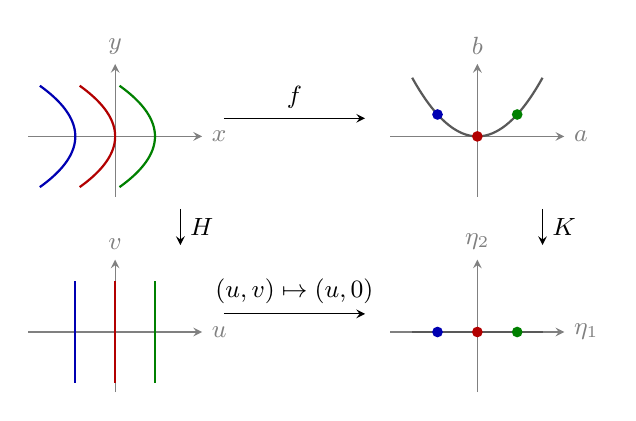
\begin{tikzpicture}[>=stealth,font=\small,scale=.92]
	\begin{scope}[yshift=2.7cm]
		\draw[->,gray] (-1.2,0)--(1.2,0) node[right] {\(x\)};
		\draw[->,gray] (0,-.83)--(0,1) node[above] {\(y\)};
		\foreach \level/\linecolour in {-.55/blue!70!black,0/red!70!black,.55/green!50!black}{
			\draw[thick,\linecolour,domain=-.7:.7,samples=40,variable=\t] plot ({\level-\t*\t},\t);
		}
	\end{scope}
	\begin{scope}[xshift=5cm,yshift=2.7cm]
		\draw[->,gray] (-1.2,0)--(1.2,0) node[right] {\(a\)};
		\draw[->,gray] (0,-.83)--(0,1) node[above] {\(b\)};
		\draw[thick,gray!70!black,domain=-.9:.9,samples=40] plot (\x,{\x*\x});
		\foreach \level/\linecolour in {-.55/blue!70!black,0/red!70!black,.55/green!50!black}{
			\fill[\linecolour] (\level,{\level*\level}) circle (2.1pt);
		}
	\end{scope}
	\draw[->] (1.5,2.95)--(3.45,2.95) node[midway,above] {\(f\)};
	\draw[->] (.9,1.7)--(.9,1.2) node[midway,right] {\(H\)};
	\draw[->] (5.9,1.7)--(5.9,1.2) node[midway,right] {\(K\)};
	\begin{scope}
		\draw[->,gray] (-1.2,0)--(1.2,0) node[right] {\(u\)};
		\draw[->,gray] (0,-.83)--(0,1) node[above] {\(v\)};
		\foreach \level/\linecolour in {-.55/blue!70!black,0/red!70!black,.55/green!50!black}{
			\draw[thick,\linecolour] (\level,-.7)--(\level,.7);
		}
	\end{scope}
	\begin{scope}[xshift=5cm]
		\draw[->,gray] (-1.2,0)--(1.2,0) node[right] {\(\eta_1\)};
		\draw[->,gray] (0,-.83)--(0,1) node[above] {\(\eta_2\)};
		\draw[thick,gray!70!black] (-.9,0)--(.9,0);
		\foreach \level/\linecolour in {-.55/blue!70!black,0/red!70!black,.55/green!50!black}{
			\fill[\linecolour] (\level,0) circle (2.1pt);
		}
	\end{scope}
	\draw[->] (1.5,.25)--(3.45,.25) node[midway,above] {\((u,v)\mapsto(u,0)\)};
\end{tikzpicture}


	\caption[常秩坐标如何同时整理原像与像]{例中的映射 \(f(x,y)=(x+y^2,(x+y^2)^2)\)。上排是原坐标，下排是经 \(H(x,y)=(x+y^2,y)\) 与 \(K(a,b)=(a,b-a^2)\) 改换后的坐标。同色源曲线映到同色目标点；新坐标使各条原像成为竖直线段，使像成为水平直线。图只显示选取的坐标范围。}
	\label{g1:fig:constant-rank-coordinates}
\end{figure}

\begin{corollary}[流形上的常秩标准形]
	\label{g1:cor:manifold-constant-rank}
	设 \(F:M^m\to N^n\) 是无边界光滑流形间的光滑映射，取 \(p\in M\)，且 \(\operatorname{rank}\mathrm{d}F_q=r\) 在 \(p\) 的某个邻域内恒定。则存在 \(p\) 与 \(F(p)\) 附近的光滑坐标，分别以这两点为原点，使 \(F\) 的坐标表达为 \((u^1,\ldots,u^m)\mapsto(u^1,\ldots,u^r,0,\ldots,0)\)，其中末尾有 \(n-r\) 个零，即\eqref{g1:eq:constant-rank-normal-form}。这里不要求坐标变化保持原先给定的度量、长度或角度。
\end{corollary}
\begin{proof}
	先选任意两张坐标图。由\cref{g1:def:manifold-differential,g1:prop:differential-chain-rule}，坐标表达的导数在两侧与坐标微分的可逆线性映射复合，所以它的秩恰为 \(\mathrm{d}F\) 的秩。Euclid 常秩定理给出源、目标坐标域中的进一步微分同胚；将它们与原坐标图复合，仍是光滑坐标图，就得到结论。构造只使用光滑可逆性，未施加任何度量限制。
\end{proof}

\subsection{秩不恒定时的反例}
\label{g1:subsec:1103:04}

常秩假设控制的是一个邻域，不是单点。单点的导数只记录一阶信息，不能独自判定附近原像的形状。不过微分矩阵的连续性确实提供一个有用的单侧结论。

\begin{proposition}
	\label{g1:prop:rank-lower-bound}
	对光滑映射 \(F:M^m\to N^n\)，若 \(\operatorname{rank}\mathrm{d}F_p\geq r\)，则在 \(p\) 的某个邻域中处处有 \(\operatorname{rank}\mathrm{d}F_q\geq r\)。特别地，若在 \(p\) 处秩达到最大可能值 \(\min(m,n)\)，则它在附近自动恒定。
\end{proposition}
\begin{proof}
	在坐标中，秩至少为 \(r>0\) 意味着某个 \(r\) 阶子式非零。该子式是导数矩阵元的多项式，随点连续，所以在足够小邻域中仍非零，秩遂仍至少为 \(r\)。当 \(r=0\) 时结论本身没有限制。最后秩始终不超过 \(\min(m,n)\)，因而达到这一上界时，邻域中的上下界相同。
\end{proof}

\begin{example}
	\label{g1:exm:cubic-rank-change}
	映射 \(f(t)=t^3\) 在原点的导数为零，在其余点的秩为 \(1\)。它仍是 \(\mathbb R\) 到自身的连续双射，逆函数为实立方根；但
	\[
		\frac{f^{-1}(h)-f^{-1}(0)}h=|h|^{-2/3}\longrightarrow\infty
		\qquad(h\to0),
	\]
	所以逆函数在零处不可微。导数可逆是局部光滑可逆的必要条件：若光滑逆存在，对两个复合恒等式求微分，便得到互逆的导数矩阵。它却不是连续可逆的必要条件，立方函数正好区分了这两件事。
\end{example}

在原点把 \(f\) 的秩记为零，并不能将立方函数在邻域中改成常值映射。任意可逆坐标变化都保持每一点的微分秩，而这个例子在任意原点邻域内都有秩为 \(1\) 的点。

\begin{example}
	\label{g1:exm:rank-changing-product}
	考虑 \(F(x,y)=(x,xy)\)，则
	\[
		\mathrm{D}F(x,y)=\begin{pmatrix}1&0\\y&x\end{pmatrix}.
	\]
	它在 \(x\ne0\) 时秩为 \(2\)，在整条 \(x=0\) 的直线上秩为 \(1\)。同值集合也发生明显变化：
	\[
		F^{-1}(a,b)=
		\begin{cases}
			\{(a,b/a)\},&a\ne0,\\
			\{(0,y):y\in\mathbb R\},&(a,b)=(0,0),\\
			\varnothing,&a=0,\ b\ne0.
		\end{cases}
	\]
	尤其在原点附近，整条短竖线被压到一点，旁边的点却各自局部可逆。若源邻域取为 \(|x|<\varepsilon,\ |y|<\delta\)，其像为
	\[
		\{(a,b):0<|a|<\varepsilon,\ |b|<\delta|a|\}\cup\{(0,0)\}.
	\]
	这个像在原点附近既不是开邻域，也不能由一段光滑坐标直线描述。常秩定理证明中的余分量在这里是 \(G(u,v)=uv\)，其 \(\mathrm{D}_vG=u\) 只在 \(u=0\) 上消失，不能因此删掉全部 \(v\) 依赖。
\end{example}

由此可见，若希望一个方程的解集或映射的原像具有稳定的局部维数，必须检查相应邻域中的正则条件。下一节将把满秩情形分别解释为浸入与淹没，并将这些坐标形式用于子流形；本节的结果只处理无边界邻域，半空间边界还需要相应的边界条件。


% !TeX root = ../../Book1.tex
% 纲要标题：### 11.4 浸入、淹没与嵌入
% 纲要位置：几何学计划纲要.md，第 558 行。
% 正文状态：初稿；尚未正式审核。

% 纲要内容开始
% 
% * 浸入和淹没的标准形
% * 正则水平集定理
% * 嵌入、初始子流形结构及限制映射
% * 单射浸入未必嵌入
% * 带边界版本中切空间与边界条件
% 
% ---
% 
% 纲要内容结束

\section{浸入、淹没与嵌入}
\label{g1:sec:1104}

第八章用秩为二的参数映射描述曲面，现在可以把同一个问题放到任意维数的流形上。一张参数片是否丢失切向方向，由微分是否单射判断；一个方程组能否在附近独立控制所有输出，由微分是否满射判断。但即使每张参数片都很规整，远处的参数仍可能回到眼前，这就需要另加拓扑条件。常秩定理先给出局部图像，嵌入的定义再保证这些局部图像与整个像的拓扑相符。本节前四个小节先讨论无边界流形，最后专门说明边界处哪些条件需要补充。

\subsection{浸入和淹没的标准形}
\label{g1:subsec:1104:01}

\begin{definition}[浸入与淹没]\label{g1:def:immersion-submersion}
	设 \(F:M^m\to N^n\) 是光滑映射。若 \(\mathrm{d}F_p:\mathrm{T}_pM\to \mathrm{T}_{F(p)}N\) 单射，称 \(F\) 在 \(p\) 处为浸入；若它满射，称 \(F\) 在 \(p\) 处为\term[yanmo]{淹没}[submersion]。处处满足相应条件时，分别称 \(F\) 为浸入或淹没。
\end{definition}

这里的浸入推广了\cref{g1:def:surface-immersion}中的曲面参数：其定义域维数为二，所以满列秩正是两个参数方向不被压在一起。一般浸入必须有 \(m\le n\)，一般淹没必须有 \(m\ge n\)。淹没也不要求映射在集合意义下满射，例如 \(t\mapsto e^t\) 是 \(\mathbb R\to\mathbb R\) 的淹没，而像只是正半轴。

\begin{theorem}[浸入与淹没的局部标准形]\label{g1:thm:immersion-submersion-normal-form}
	设 \(M^m,N^n\) 是无边界光滑流形，\(F:M\to N\) 光滑，\(p\in M\)。
	\begin{enumerate}
		\item 若 \(\mathrm{d}F_p\) 单射，则存在分别以 \(p,F(p)\) 为原点的源、目标坐标，使 \(F\) 在源的一个邻域中写成
		\[
			(u^1,\ldots,u^m)\longmapsto(u^1,\ldots,u^m,0,\ldots,0).
		\]
		\item 若 \(\mathrm{d}F_p\) 满射，则可选这样的坐标，使 \(F\) 写成
		\[
			(u^1,\ldots,u^m)\longmapsto(u^1,\ldots,u^n).
		\]
	\end{enumerate}
\end{theorem}
\begin{proof}
	单射情形，坐标 Jacobian 在 \(p\) 处有一个非零的 \(m\) 阶子式，连续性使它在某邻域内仍非零。秩又不能超过源维数 \(m\)，故该邻域的秩恒为 \(m\)。满射情形同理：一个非零的 \(n\) 阶子式保证邻域内的秩恒为 \(n\)。现在分别对秩 \(m\) 和秩 \(n\) 使用\cref{g1:cor:manifold-constant-rank}，就得到两种标准形。这里先证明邻域内秩恒定，才能调用常秩结论；仅知道一点的非极大秩，通常不能这样做。
\end{proof}

从标准形可以读出两项常用结论。浸入限制到足够小的源邻域后，是到其像的同胚：在坐标中只需投影到前 \(m\) 个坐标就得到连续逆映射。这说的是一个指定的参数分支，并没有断言其他参数分支不会进入同一个目标邻域。

\ProseParagraphBreak

无边界流形之间的淹没是开映射。事实上，把任一源开集中的点放进包含在该开集内的坐标小盒，投影标准形把这个小盒送到目标中的开盒，所有这些像的并就是原开集的像。此外，若 \(q=F(p)\)，在投影标准形中取被忘掉的坐标恒为零，就得到一个通过 \(p\) 的光滑局部截面 \(s\)，满足 \(F\circ s=\operatorname{id}\)。因此淹没允许在目标点附近光滑选择一个原像，但未必能把这些局部选择拼成全局截面。

\subsection{正则水平集定理}
\label{g1:subsec:1104:02}

方程 \(F(p)=y\) 应当减少多少自由度，取决于它实际提供了多少个独立约束。若目标维数为 \(n\)，微分满射正是所有 \(n\) 个约束在一阶上独立。淹没标准形将这个判断直接变成坐标中固定前 \(n\) 个数。

\begin{definition}[正则值]\label{g1:def:regular-value}
	设 \(F:M\to N\) 光滑。若 \(\mathrm{d}F_p\) 满射，称 \(p\) 为 \(F\) 的\term[zhengzedian]{正则点}[regular point]；否则称为\term[linjiedian]{临界点}[critical point]。若 \(y\in N\) 的每个原像都是正则点，称 \(y\) 为\term[zhengzezhi]{正则值}[regular value]；否则称为\term[linjiezhi]{临界值}[critical value]。没有原像的点也按此定义算作正则值。
\end{definition}

\begin{theorem}[正则水平集]\label{g1:thm:regular-level-set}
	设 \(F:M^m\to N^n\) 是无边界光滑流形之间的光滑映射，\(y\in N\) 是正则值。若 \(S=F^{-1}(y)\) 非空，则 \(S\) 在子空间拓扑下有自然的 \((m-n)\) 维光滑流形结构，包含映射 \(i:S\hookrightarrow M\) 是浸入，且
	\begin{equation}\label{g1:eq:regular-level-tangent}
		\mathrm{d}i_p(\mathrm{T}_pS)=\ker\mathrm{d}F_p\qquad(p\in S).
	\end{equation}
	通过单射 \(\mathrm{d}i_p\) 把 \(\mathrm{T}_pS\) 视为 \(\mathrm{T}_pM\) 的子空间时，可简写为 \(\mathrm{T}_pS=\ker\mathrm{d}F_p\)。
\end{theorem}
\begin{proof}
	对每个 \(p\in S\) 使用淹没标准形，将 \(y\) 的目标坐标取为零。在所得源坐标 \((u^1,\ldots,u^m)\) 中，水平集恰为
	\[
		u^1=\cdots=u^n=0.
	\]
	因此后 \(m-n\) 个坐标给出 \(S\) 的局部坐标，而且这些坐标与 \(S\) 的子空间拓扑一致。两张这样的坐标之间，转换映射是在环境坐标转换中先代入前 \(n\) 个坐标为零，再取所需坐标分量，故光滑；逆转换同理。这构成光滑图册。Hausdorff 性和第二可数性从环境的子空间继承，所以确实得到流形。

	在这些坐标中，包含映射的微分把后 \(m-n\) 个坐标方向单射送入 \(\mathrm{T}_pM\)。另一方面，\(\mathrm{d}F_p\) 是前 \(n\) 个方向的投影，其核恰由后 \(m-n\) 个方向张成。于是得到\eqref{g1:eq:regular-level-tangent}。坐标改变通过\cref{g1:prop:differential-chain-rule}的微分链式法则相容，所以这个子空间描述不依赖所选坐标。
\end{proof}

下一小节将通过包含映射的性质进一步说明这个自然结构为何唯一。这里并非随意给同一集合指定一种流形拓扑。只需在水平集各点满足正则值的条件，不要求 \(F\) 在整个 \(M\) 上都是淹没。

\begin{example}\label{g1:exm:regular-sphere-and-singular-level}
	设 \(F:\mathbb R^{k+1}\to\mathbb R\)，\(F(x)=\|x\|^2\)，其中 \(k\ge1\)。因为
	\[
		\mathrm{d}F_x(v)=2\langle x,v\rangle,
	\]
	每个 \(c>0\) 都是正则值，球面 \(F^{-1}(c)\) 的维数为 \(k\)，并且 \(\mathrm{T}_xF^{-1}(c)=x^\perp\)。负数也为正则值，但水平集为空。零为临界值，其水平集只有一个点；该集合仍可以是零维流形，却不具有正则水平集定理所给的预期维数 \(k\)。

	另取 \(G(x,y)=xy\)。它的零水平集是两条坐标轴的并，在原点形成四条分支，不是原点附近的一维流形。两个例子说明：临界水平集有时仍规整，有时出现交叉，仅由“不是正则值”不能断言所有水平集具有同一种奇异性。
\end{example}

\subsection{嵌入、初始子流形结构及限制映射}
\label{g1:subsec:1104:03}

第四章的拓扑嵌入要求映射与其像之间互为连续逆映射，像必须使用环境的子空间拓扑。加入这个条件以后，浸入的局部参数片才会与整个像的局部邻域一致。

\begin{definition}[光滑嵌入]\label{g1:def:smooth-embedding}
	无边界光滑流形之间的光滑映射 \(f:M\to N\)，若既是浸入，又是 \(M\) 到 \(f(M)\) 的同胚，其中 \(f(M)\) 取 \(N\) 的子空间拓扑，则称为\term[guanghuaqianru]{光滑嵌入}[smooth embedding]，简称嵌入。
\end{definition}

\begin{definition}[嵌入子流形]\label{g1:def:embedded-submanifold}
	设 \(N^n\) 为无边界光滑流形。子集 \(S\subset N\) 若对每个 \(p\in S\) 都有环境坐标 \((V,y)\)，使
	\[
		y(S\cap V)=y(V)\cap\bigl(\mathbb R^k\times\{0\}^{n-k}\bigr),
	\]
	则称为 \(N\) 的 \(k\) 维\term[qianruziliuxing]{嵌入子流形}[embedded submanifold]。给 \(S\) 子空间拓扑，并用这些切片的前 \(k\) 个坐标作为图册。
\end{definition}

坐标切片之间的转换正如正则水平集证明中那样光滑，所以这个定义确实给出 \(S\) 的光滑结构。下述等价关系说明，这个集合式定义与前面的映射式定义对应。

\begin{proposition}[嵌入与坐标切片]\label{g1:prop:embedding-slice-characterization}
	设 \(M^k,N^n\) 是无边界光滑流形。若 \(f:M\to N\) 为光滑嵌入，则其像 \(S=f(M)\) 为嵌入子流形，且 \(f:M\to S\) 是微分同胚。反之，每个嵌入子流形的包含映射都是光滑嵌入。
\end{proposition}
\begin{proof}
	取 \(p\in M\)，浸入标准形给出源邻域 \(U\) 及 \(f(p)\) 附近的坐标，使 \(f|_U\) 的像是一块坐标切片。必要时缩小坐标盒，可以使这块切片完整覆盖目标小盒中的前 \(k\) 个坐标。关键是排除 \(M\setminus U\) 的点也映入眼前的小盒：因为 \(f\) 是到子空间 \(S\) 的同胚，\(f(U)\) 在 \(S\) 中开，故存在环境开集 \(W\subset N\)，满足 \(S\cap W=f(U)\)。把目标坐标盒进一步缩到 \(W\) 内，盒内的整个 \(S\) 就恰为该切片，而不只是其中一个参数分支。这样的盒覆盖 \(S\)，给出嵌入子流形结构。在对应坐标中，\(f:M\to S\) 是恒等坐标映射，故连同逆映射都光滑。

	反过来，包含映射在适配坐标中为 \(u\mapsto(u,0)\)，所以是浸入。\(S\) 已取环境的子空间拓扑，包含映射自然是到其像的同胚，故为光滑嵌入。
\end{proof}

\begin{proposition}[嵌入子流形的初始性质]\label{g1:prop:embedded-initial-property}
	设 \(S\subset N\) 为无边界光滑流形 \(N\) 的嵌入子流形，\(i:S\hookrightarrow N\) 为包含映射。对任意光滑流形 \(P\)（允许有边界）及任意集合映射 \(h:P\to S\)，有
	\[
		h:P\to S\text{ 光滑}\quad\Longleftrightarrow\quad i\circ h:P\to N\text{ 光滑}.
	\]
	特别地，光滑映射 \(H:P\to N\) 若像包含在 \(S\) 中，就唯一地给出光滑映射 \(P\to S\)。在固定子集 \(S\subset N\) 上，使其成为嵌入子流形的光滑结构唯一。
\end{proposition}
\begin{proof}
	正向由光滑映射的复合得到。反向先处理一个容易遗漏的拓扑问题：若 \(i\circ h\) 光滑，则它连续；由于 \(S\) 取子空间拓扑，\(h\) 也连续。于是对 \(h(p)\) 附近的适配图 \(V\)，集合 \(h^{-1}(S\cap V)\) 在 \(P\) 中开。在这片上，\(h\) 的坐标表示就是 \(i\circ h\) 的坐标表示的前 \(\dim S\) 个分量，所以光滑。即使 \(p\) 在 \(\partial P\)，这些分量仍由环境中的光滑延拓限制得到，论证不变。局部结论合起来给出 \(h\) 光滑。

	像包含在 \(S\) 的映射只有一种集合意义下的限制值域方式，上述等价立即证明其光滑性。若同一个子集带有两种嵌入子流形结构，两种包含映射都光滑。对两种结构之间的恒等集合映射分别使用已证等价，得到恒等映射在两个方向都光滑，故两种极大光滑图册相同。
\end{proof}

这里的“初始”说的是通过包含映射检测光滑性的性质，不是另给 \(S\) 加一种比子空间拓扑更细的拓扑。例如光滑函数 \(f:N\to\mathbb R\) 限制到 \(S\) 后光滑；若 \(f(S)\subset T\)，其中 \(T\) 也是嵌入子流形，则 \(f|_S:S\to T\) 光滑。正则水平集由环境坐标切片构造，因而属于这一情形。

\ProseParagraphBreak

包含映射的微分通常被省略在记号里：对嵌入子流形写 \(\mathrm{T}_pS\subset \mathrm{T}_pN\)，实际是用单射 \(\mathrm{d}i_p\) 作识别。这不是把两个定义不同的导子集合逐项当作相同集合，而是利用包含映射，在前者与后者的一个子空间之间建立自然的线性同构。

\subsection{单射浸入未必嵌入}
\label{g1:subsec:1104:04}

单射解决了“一个像点有几个原像”，却没有解决“附近像点的原像是否也在附近”。下面的平面曲线已经能把两者区别开，不需要依靠高维或稠密轨道的例子。

\begin{example}\label{g1:exm:injective-immersion-not-embedding}
	令
	\[
		\gamma:(-\pi,\pi)\longrightarrow\mathbb R^2,
		\qquad\gamma(t)=(\sin t,\sin2t).
	\]
	它是单射浸入，但不是嵌入。先检查浸入：\(\gamma'(t)=(\cos t,2\cos2t)\)，若第一分量为零，则 \(t=\pm\pi/2\)，第二分量为 \(-2\ne0\)，故导数从不为零。

	再检查单射。\(\sin t\) 的正负区分正、负参数，且在本区间内只在 \(t=0\) 为零。若 \(s,t\in(0,\pi)\) 且 \(\sin s=\sin t\)，则 \(s=t\) 或 \(s=\pi-t\)；后一情形的 \(\sin2s=-\sin2t\)，两者相等只能有 \(t=\pi/2\)，此时仍为 \(s=t\)。负参数的情形用 \(\gamma(-t)=-\gamma(t)\) 化为正参数，因而 \(\gamma\) 单射。

	然而取 \(t_j\to\pi\)，便有 \(\gamma(t_j)\to(0,0)=\gamma(0)\)，而 \(t_j\) 不趋于零。因此从像的子空间拓扑返回参数的逆映射不连续。\cref{g1:fig:injective-immersion-topology}中，蓝色短弧来自零附近的参数，另一方向逼近交点的曲线来自接近参数区间端点的部分。浸入标准形只能控制前一支。

	这个像甚至是闭集：把同一公式延拓到紧区间 \([-\pi,\pi]\)，两个端点都映到已有的 \(\gamma(0)\)，所以延拓前后的像相同，是紧集。可见“单射浸入且像闭”仍不能替代嵌入条件。
\end{example}

% !TeX root = ../Book1.tex
\begin{figure}[htbp]
	\centering
	\begin{tikzpicture}[font=\small]
		\begin{scope}[xshift=-2.8cm,x=2cm,y=1.3cm]
			\draw[->,GeometryGray] (-1.25,0)--(1.3,0) node[right] {\(x\)};
			\draw[->,GeometryGray] (0,-1.2)--(0,1.25) node[above] {\(y\)};
			\draw[GeometryGray,thick,domain=-180:180,samples=181,variable=\t] plot ({sin(\t)},{sin(2*\t)});
			\draw[GeometryBlue,very thick,domain=-27:27,samples=40,variable=\t] plot ({sin(\t)},{sin(2*\t)});
			\draw[orange!75!black,very thick,domain=145:179.8,samples=35,variable=\t] plot ({sin(\t)},{sin(2*\t)});
			\foreach \t in {150,165,174,178}{\fill[orange!75!black] ({sin(\t)},{sin(2*\t)}) circle (1.25pt);}
			\fill[GeometryBlue] (0,0) circle (1.6pt);
			\node[above left] at (0,0) {\(\gamma(0)\)};
			\node[GeometryBlue,above right] at (0.5,0.78) {\(t\approx0\)};
			\node[orange!75!black,right] at (0.63,-0.72) {\(t\uparrow\pi\)};
		\end{scope}
		\begin{scope}[xshift=3.7cm,yshift=0.2cm]
			\draw[GeometryGray] (-1.7,0)--(1.7,0);
			\draw[fill=white] (-1.7,0) circle (2pt);
			\draw[fill=white] (1.7,0) circle (2pt);
			\fill[GeometryBlue] (0,0) circle (2pt);
			\node[below] at (-1.7,0) {\(-\pi\)};
			\node[below] at (0,0) {\(0\)};
			\node[below] at (1.7,0) {\(\pi\)};
			\foreach \x in {1,1.35,1.52,1.61}{\fill[orange!75!black] (\x,0) circle (1.5pt);}
			\draw[->,orange!75!black] (0.95,0.35)--(1.65,0.35);
			\node[above] at (0,0.75) {参数区间 \((-\pi,\pi)\)};
			\node[align=center] at (0,-1) {\(\gamma(t_j)\to\gamma(0)\)\\但 \(t_j\not\to0\)};
		\end{scope}
	\end{tikzpicture}
	\caption[单射浸入的像拓扑]{曲线 \(\gamma(t)=(\sin t,\sin2t)\)，定义域为 \((-\pi,\pi)\)。蓝色弧是零附近的参数片；橙色点来自趋向 \(\pi\) 的参数，也在像中趋向原点。逆参数映射因而不连续，尽管每个参数点的导数非零且参数映射单射。}
	\label{g1:fig:injective-immersion-topology}
\end{figure}


还可以在这个例子中具体看出，嵌入子流形的初始性质不能自动移植给任意单射浸入像。给集合 \(S=\gamma((-\pi,\pi))\) 从参数区间搬来流形结构，使 \(\gamma\) 成为微分同胚；此时包含 \(S\to\mathbb R^2\) 是浸入。对充分小的 \(\varepsilon>0\)，考虑值在 \(S\) 中的曲线
\[
	h(s)=(-\sin s,\sin2s),\qquad |s|<\varepsilon.
\]
作为到 \(\mathbb R^2\) 的映射，它光滑；但它在 \(S\) 的参数坐标为
\[
	\gamma^{-1}(h(s))=
	\begin{cases}
		\pi+s,&s<0,\\
		0,&s=0,\\
		-\pi+s,&s>0,
	\end{cases}
\]
在零处不连续，故 \(h:(-\varepsilon,\varepsilon)\to S\) 不是光滑映射。问题恰是这份流形结构的拓扑不同于 \(S\) 的子空间拓扑。

\begin{definition}[固有映射]\label{g1:def:proper-map-manifolds}
	光滑流形之间的连续映射 \(f:M\to N\) 若对每个紧集 \(K\subset N\)，原像 \(f^{-1}(K)\) 都紧，则称为\term[guyouyingshe]{固有映射}[proper map]。
\end{definition}

固有性控制的是“落在一个固定紧目标区域内的所有参数”。上一例中整个像紧，而其原像是非紧区间 \((-\pi,\pi)\)，所以 \(\gamma\) 不固有。这一条件能排除远处参数悄悄回到紧区域的现象。

\begin{proposition}[固有单射浸入]\label{g1:prop:proper-injective-immersion}
	设 \(M,N\) 为无边界光滑流形，\(f:M\to N\) 为单射浸入。若 \(f\) 固有，则 \(f\) 是嵌入，且像闭于 \(N\)。特别地，若 \(M\) 紧，则每个单射浸入 \(M\to N\) 都是闭像嵌入。反之，闭像嵌入是固有映射。
\end{proposition}
\begin{proof}
	先证明一个连续固有映射 \(f:M\to N\) 是闭映射。取闭集 \(A\subset M\) 及 \(y\in\overline{f(A)}\)。在 \(N\) 的坐标图内取一个紧邻域 \(K\ni y\)，使 \(y\in\operatorname{int}K\)。固有性使 \(f^{-1}(K)\) 紧，故其闭子集 \(A\cap f^{-1}(K)\) 紧。它的连续像
	\[
		f(A\cap f^{-1}(K))=f(A)\cap K
	\]
	也紧，并由\cref{g1:prop:compact-hausdorff-closed}闭于 \(N\)。回忆这里闭性的理由：对紧集外一点，用 Hausdorff 性把它与紧集的每一点用开邻域分开，再以有限子覆盖替代紧集一侧的全部邻域，取外点一侧有限个邻域的交，便得到与紧集不交的开邻域。因为 \(y\) 位于 \(K\) 的内部且是 \(f(A)\) 的闭包点，它也是 \(f(A)\cap K\) 的闭包点，因而属于该闭集。于是 \(f(A)\) 闭。

	现在 \(f\) 连续且单射，并将闭集送到闭集，所以 \(f:M\to f(M)\) 的逆映射连续。它又是浸入，故为嵌入；取 \(A=M\) 还得到像闭。若 \(M\) 紧，每个目标紧集在 Hausdorff 空间 \(N\) 中闭，其原像为 \(M\) 的闭子集，因而紧，所以 \(f\) 自动固有。此时也可直接使用\cref{g1:thm:compact-bijection}判断到像的逆连续。

	反之，若 \(f\) 是闭像嵌入，则 \(K\cap f(M)\) 对每个紧 \(K\subset N\) 都是紧集；由同胚 \(M\cong f(M)\)，其原像 \(f^{-1}(K)\) 紧，故 \(f\) 固有。
\end{proof}

并非所有嵌入都固有。例如开区间 \((0,1)\hookrightarrow\mathbb R\) 是嵌入，但紧集 \([0,1]\) 的原像不紧。固有单射浸入给出的是一种保证闭像嵌入的充分判据，并没有把“嵌入”的含义改成“闭子集”。

\subsection{带边界版本中切空间与边界条件}
\label{g1:subsec:1104:05}

对带边界流形，浸入、淹没仍按完整微分的单射、满射定义，嵌入仍要求同时是浸入和到子空间像的同胚。边界坐标采用 \(\mathbb H^m=\{x^m\ge0\}\)。\cref{g1:prop:derivation-coordinate-basis}及\cref{g1:prop:boundary-velocities}说明，即使 \(p\in\partial M\)，完整切空间 \(\mathrm{T}_pM\) 仍是 \(m\) 维向量空间；向内半空间只是其中能够由向内单侧曲线实现的速度集合，不能代替整个切空间。若以 \(\rho=x^m\) 为局部边界定义函数，则
\[
	\mathrm{T}_p(\partial M)=\ker\mathrm{d}\rho_p\subset \mathrm{T}_pM.
\]
边界上各种满秩条件因此仍按完整切空间计算，但由此得到的 Euclid 局部变换未必保留半空间。

\begin{proposition}[边界处的局部逆]\label{g1:prop:boundary-local-inverse}
	设 \(M^m,N^m\) 为带边界光滑流形，\(m\ge1\)，\(F:M\to N\) 光滑。若 \(p\in\partial M\)、\(F(p)\in\partial N\)，在 \(p\) 的某邻域内有 \(F(\partial M)\subset\partial N\)，并且 \(\mathrm{d}F_p\) 可逆，则 \(F\) 限制到 \(p\) 的某个相对开邻域后，是到 \(F(p)\) 的一个相对开邻域的微分同胚。
\end{proposition}
\begin{proof}
	取两边的半空间坐标，把 \(p,F(p)\) 都置于零。按边界光滑映射的定义，坐标表示 \(G\) 可光滑延拓到 \(\mathbb R^m\) 的一个开邻域。保边界条件给出 \(G^m(x',0)=0\)，所以由一元微积分基本定理，
	\[
		G^m(x',x^m)=x^m a(x',x^m),\qquad
		a(x',x^m)=\int_0^1\partial_mG^m(x',t x^m)\,\mathrm{d}t.
	\]
	\(\mathrm{d}G_0\) 的最后一行在前 \(m-1\) 列为零；可逆性因而使 \(a(0)\ne0\)。又因为 \(G\) 把 \(x^m\ge0\) 的点送到目标半空间，一侧导数给出 \(a(0)\ge0\)，故 \(a(0)>0\)。缩小邻域使 \(a>0\)，则 \(G^m\) 与 \(x^m\) 同号。对 Euclid 延拓使用\cref{g1:thm:inverse-function}，得到开邻域间的光滑逆；同号性质说明该逆也保留半空间。把这对互逆映射限制到半空间，便得到所需边界局部逆。
\end{proof}

保边界条件不能只检查在一个点成立。例如
\[
	G:\mathbb H^2\to\mathbb H^2,\qquad G(x,y)=(x,y+x^2)
\]
在原点的微分是恒等映射，也把原点送到原点，但它把附近的边界点送到抛物线 \(v=u^2\)。其像在 \(v\ge u^2\) 中，不包含原点在目标半平面中的任何相对开邻域，所以不是边界局部微分同胚。Euclid 延拓的逆 \((u,v)\mapsto(u,v-u^2)\) 光滑，却未必取值于源半平面。

\ProseParagraphBreak

对水平集，正确的附加条件要求约束在边界切向方向中仍然独立。这样，约束不会把唯一的向内方向全部吃掉。若带边界子流形 \(S\subset M\) 满足 \(\partial S=S\cap\partial M\)，且在这些点满足
\[
	\mathrm{T}_pS+\mathrm{T}_p(\partial M)=\mathrm{T}_pM,
\]
本书用\term[neatziliuxing]{与边界相容的横截嵌入子流形}[neat submanifold]描述同时满足这两个条件的子流形。这里包含映射要求为嵌入；横截等式意味着 \(\mathrm{T}_pS\) 中还保留至少一个不沿环境边界的方向。

\begin{theorem}[带边界的正则水平集]\label{g1:thm:boundary-regular-level-set}
	设 \(M^m\) 为带边界光滑流形，\(N^n\) 为无边界光滑流形，\(F:M\to N\) 光滑。若 \(y\in N\) 同时为 \(F\) 及 \(F|_{\partial M}\) 的正则值，则非空水平集 \(S=F^{-1}(y)\) 自然成为 \((m-n)\) 维带边界嵌入子流形，且
	\[
		\partial S=S\cap\partial M,\qquad \mathrm{T}_pS=\ker\mathrm{d}F_p.
	\]
	它是与边界相容的横截嵌入子流形；在边界点还满足
	\[
		\mathrm{T}_p(\partial S)=\ker\mathrm{d}F_p\cap \mathrm{T}_p(\partial M).
	\]
\end{theorem}
\begin{proof}
	内部点使用\cref{g1:thm:regular-level-set}的局部证明。取 \(p\in S\cap\partial M\)，用半空间坐标将 \(p\) 置于零，用目标坐标将 \(y\) 置于零，记映射的坐标分量为 \(f^1,\ldots,f^n\)。\(F|_{\partial M}\) 在 \(p\) 处满秩，意味着 Jacobian 的前 \(m-1\) 列中有一个非零的 \(n\) 阶子式。重排前 \(m-1\) 个坐标，可令该子式来自前 \(n\) 列。特别地，若水平集碰到边界，必有 \(m-n\ge1\)。

	对 \(f\) 的 Euclid 光滑延拓构造
	\[
		\Phi(x)=\bigl(f^1(x),\ldots,f^n(x),x^{n+1},\ldots,x^{m-1},x^m\bigr).
	\]
	\(\mathrm{d}\Phi_0\) 可逆，故由\cref{g1:thm:inverse-function}，它在足够小的 Euclid 开邻域间为微分同胚。与任意使用常秩定理不同，这里特意把最后一个坐标原样保留：\(\Phi^m(x)=x^m\)。因此 \(\Phi\) 及其逆都保留半空间和边界。以 \(u=\Phi(x)\) 为新的边界坐标，水平集成为
	\begin{equation}\label{g1:eq:boundary-level-slice}
		u^1=\cdots=u^n=0,\qquad u^m\ge0.
	\end{equation}
	后 \(m-n\) 个坐标给出水平集的半空间图，其边界恰是 \(u^m=0\)，也就是环境边界与水平集的交。图册转换由环境光滑转换的限制得到，子空间拓扑、Hausdorff 性及第二可数性同无边界情形，因此得到带边界嵌入子流形。

	在这些坐标中，\(\mathrm{T}_pS\) 由后 \(m-n\) 个完整坐标方向张成，等于 \(\ker\mathrm{d}F_p\)；其边界切空间再去掉最后一个方向，正是 \(\ker\mathrm{d}F_p\cap \mathrm{T}_p(\partial M)\)。最后一个方向 \(\partial/\partial u^m\) 属于 \(\mathrm{T}_pS\) 却不属于 \(\mathrm{T}_p(\partial M)\)，而后者余维为一，故两者之和为整个 \(\mathrm{T}_pM\)。这就同时验证了边界交等式与横截条件。
\end{proof}

上述半空间切片还说明，与边界相容的横截水平集仍具有初始性质：一个映射若值在 \(S\) 中，其是否光滑可以通过组合包含 \(S\hookrightarrow M\) 来检验。证明仍先用子空间拓扑得到连续性，再取\eqref{g1:eq:boundary-level-slice}中后 \(m-n\) 个坐标；这些坐标有环境光滑延拓，因此同样适用于带边界的源。

\ProseParagraphBreak

只检查完整切空间上的 \(\mathrm{d}F\) 满射还不够。例如 \(F:\mathbb H^m\to\mathbb R\)，\(F(x)=x^m\)，处处满秩，但 \(F^{-1}(0)=\partial M\) 是一张无边界的 \((m-1)\) 维流形；其自身边界为空，而与 \(\partial M\) 的交却是整个水平集，故不是 与边界相容的横截水平集。更明显地，\(F(x,y)=y+x^2\) 在 \(\mathbb H^2\) 上也处处满秩，但零水平集只有原点，连预期的一维局部形状都没有。两例中 \(F|_{\partial M}\) 都在相关点失去满秩性，正是附加条件所要排除的现象。


\begin{chaptersummary}
	光滑结构由两两相容的坐标图确定，坐标图的极大扩张消除了任意多列或少列相容图的区别。球面和射影空间可以直接用图册构造；同一个底层拓扑却不能独自决定哪些函数光滑。边界图使用半空间中的局部延拓，延拓函数可以不同，但边界点处各阶导数相同。

	\ProseParagraphBreak

	切向量是作用于局部函数芽的一阶导子，坐标导数给出它的基。内点处每个切向量都能由双侧曲线实现；边界处双侧速度只给出边界切空间，单侧速度给出内向锥，完整切空间仍为 \(n\) 维。切丛把不同点的切空间通过微分换坐标组织在一起；光滑映射的微分向前送切向量，其对偶反向拉回余切向量。

	\ProseParagraphBreak

	逆函数定理以可逆线性近似控制非线性余项，通过压缩迭代产生局部逆。隐函数定理把待求变量与参数一起放入这一构造；常秩定理再利用秩在邻域中不变，消去剩余坐标的变化，得到局部投影或坐标包含。满秩约束因此给出光滑水平集，切空间正是约束微分的核。

	\ProseParagraphBreak

	浸入只控制局部切方向，嵌入还要求源拓扑与像的子空间拓扑相符；单射和闭像各自都不足以代替这一条件，固有性则提供实用的充分条件。边界问题还必须辨认边界是否对应、约束是否沿边界仍满秩。Euclid 延拓的局部可逆，不会自动保证它的逆留在所需的半空间一侧。
\end{chaptersummary}

\BookExercises


\begin{exercise}
	\label{g1:ex:stereographic-smooth-charts}
	设 \(n\geq1\)，\(N=(0,\ldots,0,1)\)、\(S=-N\) 是 \(S^n\) 的两极。对 \(x=(x',x_{n+1})\) 定义
	\[
		\sigma_N(x)=\frac{x'}{1-x_{n+1}},\qquad
		\sigma_S(x)=\frac{x'}{1+x_{n+1}}.
	\]
	求这两个映射的逆，证明它们给出与\cref{g1:exm:sphere-smooth-atlas}相同的光滑结构，并求换坐标 \(\sigma_S\circ\sigma_N^{-1}\)。说明换坐标在零点没有定义的几何原因。
\end{exercise}

\begin{solution}
	解 \(u=x'/(1-x_{n+1})\) 与 \(|x'|^2+x_{n+1}^2=1\)，得到
	\[
		\sigma_N^{-1}(u)=\left(\frac{2u}{1+|u|^2},\frac{|u|^2-1}{1+|u|^2}\right),\qquad
		\sigma_S^{-1}(v)=\left(\frac{2v}{1+|v|^2},\frac{1-|v|^2}{1+|v|^2}\right).
	\]
	这些式子对任意 \(u,v\in\mathbb R^n\) 有意义，代回即得到恒等式，且与原映射均连续。因此它们分别是 \(S^n\setminus\{N\}\)、\(S^n\setminus\{S\}\) 到 \(\mathbb R^n\) 的坐标图。与正文半球图转换时，一向由上述有理式后删除一个分量得到，另一向由半球图的光滑平方根表达代入 \(\sigma_N\) 或 \(\sigma_S\) 得到，分母在相应交叠处非零，故两种图册相容。

	在 \(u\neq0\) 时，把逆式代入可得
	\[
		(\sigma_S\circ\sigma_N^{-1})(u)=\frac{u}{|u|^2}.
	\]
	该映射的逆仍是自身。\(u=0\) 在北极投影图中代表南极，而南极不属于另一张图的图域，故这里的未定义来自图域没有交叠，并非球面的奇点。
\end{solution}

\begin{exercise}
	\label{g1:ex:projective-line-circle}
	证明映射
	\[
		F:\mathbb{RP}^1\longrightarrow S^1,\qquad
		F([x:y])=\left(\frac{x^2-y^2}{x^2+y^2},\frac{2xy}{x^2+y^2}\right)
	\]
	是微分同胚。要求直接给出局部逆的坐标公式，不只利用紧空间到 Hausdorff 空间的连续双射性质。
\end{exercise}

\begin{solution}
	两个分式在同时缩放 \((x,y)\) 后不变，且其平方和为 \(1\)，所以 \(F\) 良定义。在图 \(x\neq0\) 中写 \(t=y/x\)，有
	\[
		F([1:t])=\left(\frac{1-t^2}{1+t^2},\frac{2t}{1+t^2}\right).
	\]
	它的像为圆周除去 \((-1,0)\)，逆坐标为 \(t=b/(1+a)\)，其中 \((a,b)\in S^1\)、\(a\neq-1\)。在图 \(y\neq0\) 中写 \(s=x/y\)，得到
	\[
		F([s:1])=\left(\frac{s^2-1}{s^2+1},\frac{2s}{s^2+1}\right),\qquad s=\frac{b}{1-a}\quad(a\neq1).
	\]
	两组逆式覆盖整个圆周。在同时有定义处，\(st=b^2/((1-a)(1+a))=1\)，所以它们给出同一射影点。两组公式还证明满射与单射；正文的球面图与射影图中各式都光滑，因此 \(F\) 及其逆光滑。
\end{solution}

\begin{exercise}
	\label{g1:ex:transported-line-powers}
	对正奇数 \(r\)，在通常拓扑的 \(\mathbb R\) 上用全局坐标 \(u_r(t)=t^r\) 定义光滑流形 \(M_r\)。对两个正奇数 \(r,s\)，判断集合恒等映射 \(I_{r,s}:M_r\to M_s\) 何时光滑、何时为微分同胚。证明无论 \(r,s\) 如何，\(M_r\) 与 \(M_s\) 总微分同胚。
\end{exercise}

\begin{solution}
	恒等映射的坐标表达为 \(u\mapsto\operatorname{sgn}(u)|u|^{s/r}\)。若 \(s/r\) 是整数，由 \(r,s\) 都为奇数知它是正奇数，表达式就是光滑多项式 \(u^{s/r}\)。若 \(\alpha=s/r\) 不是整数，取 \(k=\lfloor\alpha\rfloor+1\)，在正半轴上第 \(k\) 阶导数等于非零常数乘 \(u^{\alpha-k}\)，当 \(u\downarrow0\) 时无界，因此不可能在零点 \(C^k\)，更不光滑。故 \(I_{r,s}\) 光滑当且仅当 \(r\) 整除 \(s\)；正反两个恒等映射同时光滑当且仅当 \(r=s\)。

	不过映射 \(F=u_s^{-1}\circ u_r:M_r\to M_s\) 始终是微分同胚，因为 \(u_s\circ F\circ u_r^{-1}\) 为恒等映射，逆也一样。具体集合公式为 \(F(t)=\operatorname{sgn}(t)|t|^{r/s}\)。这个公式在通常坐标中可能不光滑，并不妨碍它在指定的源、目标结构之间成为微分同胚。
\end{solution}

\begin{exercise}
	\label{g1:ex:boundary-even-extension}
	设 \(f:[0,\infty)\to\mathbb R\) 按局部延拓意义光滑。证明偶延拓 \(E_f(t)=f(|t|)\) 在 \(\mathbb R\) 上光滑，当且仅当 \(f^{(2j+1)}(0)=0\) 对所有 \(j\geq0\) 成立。再构造一个在负半轴不恒为零的光滑函数 \(h:\mathbb R\to\mathbb R\)，使 \(h\) 在非负半轴恒为零，解释为什么边界处各阶导数的唯一性不意味着延拓函数唯一。
\end{exercise}

\begin{solution}
	如果 \(E_f\) 光滑，由它是偶函数可得 \(E_f^{(k)}(0)=(-1)^kE_f^{(k)}(0)\)，故所有奇阶导数为零；在右侧这些导数就是 \(f\) 的边界导数。

	反过来，假设所有奇阶边界导数为零。在正、负半轴上，\(E_f\) 的第 \(k\) 阶导数分别是 \(f^{(k)}(t)\)、\((-1)^kf^{(k)}(-t)\)。当 \(k\) 为偶数时两边极限相同，为奇数时两边极限均为零，故每一阶候选导数均可连续粘合。为确认它们确为导数，依次用微积分基本定理：若第 \(k+1\) 阶候选函数连续，则其从 \(0\) 到 \(t\) 的积分在两侧都等于第 \(k\) 阶候选函数减去其零点值，因而第 \(k\) 阶候选函数在零点也可微。对任意有限阶重复这一论证，得到 \(E_f\in C^\infty\)。例如 \(f(t)=t^2\) 的偶延拓光滑，\(f(t)=t\) 的偶延拓则是 \(|t|\)，在零点不可微。

	取 \(h(t)=e^{-1/t^2}\) 当 \(t<0\)，\(h(t)=0\) 当 \(t\geq0\)。每次在负半轴求导，都得到一个关于 \(1/t\) 的多项式乘 \(e^{-1/t^2}\)。由 \(u^Ne^{-u^2}\to0\)（\(u\to\infty\)）对每个 \(N\) 成立，这些导数以及它们除以 \(t\) 后的极限均为零，归纳可知零点的各阶导数存在且为零。因此 \(h\) 光滑而不恒为零。对任何一个已取的光滑延拓 \(\widetilde f\)，\(\widetilde f+c h\) 在共同定义的邻域上都是另一个延拓；所有边界导数相同，负半轴上的值却可不同。
\end{solution}
\begin{exercise}
	\label{g1:ex:point-derivation-orders}
	对实直线零点处的光滑函数芽，固定 \(a,b,c\in\mathbb R\)，令
	\[
		L(f)=a f(0)+b f'(0)+c f''(0).
	\]
	求出使 \(L\) 成为零点处导子的全部系数组合，并说明本题为什么体现了导子只记录一阶变化。
\end{exercise}
\begin{solution}
	导子必消去常数，对 \(f=1\) 得 \(a=0\)。再取 \(f(x)=g(x)=x\)，因为 \(f(0)=g(0)=0\)，乘法法则要求 \(L(x^2)=0\)。左边等于 \(2c\)，所以 \(c=0\)。系数 \(b\) 则不受限制：普通求导的乘法法则说明 \(L(f)=b f'(0)\) 对任意 \(b\in\mathbb R\) 都是导子。

	所以全部解是 \((a,b,c)=(0,b,0)\)。零阶求值项被 \(L(1)=0\) 排除，二阶项则被两个在该点为零的函数相乘排除。二阶导数的乘积公式含有额外交叉项 \((fg)''(0)=f''(0)g(0)+2f'(0)g'(0)+f(0)g''(0)\)，因此不满足点导子的乘法法则。
\end{solution}

\begin{exercise}
	\label{g1:ex:sphere-derivation-tangent}
	单位球面 \(S^2\subset\mathbb R^3\) 取标准光滑结构，\(\iota:S^2\to\mathbb R^3\) 为包含映射。用本节的导子或曲线定义证明 \(\mathrm{d}\iota_p\) 单射，且
	\[
		\mathrm{d}\iota_p(\mathrm{T}_pS^2)=\{w\in\mathbb R^3:\langle p,w\rangle=0\}.
	\]
	在这个识别下求对径映射 \(A(p)=-p\) 的微分，以及高度函数 \(h(p)=p_3\) 的微分；找出 \(\mathrm{d}h_p=0\) 的点。
\end{exercise}
\begin{solution}
	记环境坐标限制到球面的函数为 \(x_1,x_2,x_3\)。切向量 \(v\in \mathrm{T}_pS^2\) 的像为 \(w=(v(x_1),v(x_2),v(x_3))\)。对函数恒等式 \(\sum_i x_i^2=1\) 作用导子，得 \(2\sum_i p_iw_i=0\)，故像包含在正交平面内。

	选 \(i\) 使 \(p_i\ne0\)。在 \(p\) 的小邻域内，另外两个环境坐标是球面坐标，遗漏的一项由
	\[
		x_i=\operatorname{sgn}(p_i)\sqrt{1-\sum_{j\ne i}x_j^2}
	\]
	恢复。若 \(\mathrm{d}\iota_p(v)=0\)，则 \(v\) 作用于这两个局部坐标均为零，坐标基公式迫使 \(v=0\)，所以微分单射。任意 \(w\perp p\)、\(w\ne0\) 又可由球面曲线
	\[
		\gamma(t)=p\cos(|w|t)+\frac{w}{|w|}\sin(|w|t)
	\]
	实现：由 \(|p|=1\)、\(p\perp w\) 可知 \(|\gamma(t)|=1\)，且 \(\gamma(0)=p\)、\(\gamma'(0)=w\)。\(w=0\) 用常值曲线实现。因此所述平面恰为全部像。

	对径映射把代表曲线 \(\gamma\) 送到 \(-\gamma\)，所以 \(\mathrm{d}A_p(w)=-w\in \mathrm{T}_{-p}S^2\)。虽然两个切平面在环境中是同一个线性子空间，它们作为切丛的纤维仍有不同基点。高度微分为 \(\mathrm{d}h_p(w)=w_3\)。它在全部 \(w\perp p\) 上为零，当且仅当 \(e_3=(0,0,1)\) 与 \(p\) 平行，故恰在南北两极 \((0,0,\pm1)\) 为零。
\end{solution}

\begin{exercise}
	\label{g1:ex:circle-tangent-trivialization}
	圆周 \(S^1=\{(x,y):x^2+y^2=1\}\) 取标准角坐标。对 \(p=(x,y)\) 及 \(s\in\mathbb R\)，令 \(v_{p,s}\) 为曲线 \(t\mapsto R_{st}p\) 在零时刻的速度，其中 \(R_\theta\) 是平面旋转。证明
	\[
		\Psi:S^1\times\mathbb R\longrightarrow \mathrm{T}S^1,\qquad
		\Psi(p,s)=v_{p,s}
	\]
	是微分同胚。再将 \(S^1\) 记成复数单位圆，求映射 \(F_k(z)=z^k\)、\(k\in\mathbb Z\) 在这一表示下的切映射。
\end{exercise}
\begin{solution}
	在局部角坐标 \(p=(\cos\theta,\sin\theta)\) 中，曲线 \(R_{st}p\) 的角度为 \(\theta+st\)，所以 \(v_{p,s}=s\partial_\theta|_p\)。切空间一维，故每个 \(v\in \mathrm{T}_pS^1\) 都有且仅有一个这样的 \(s\)。因此 \(\Psi\) 双射。角度换成 \(\theta+2\pi m\) 不改变 \(\partial_\theta\) 或系数 \(s\)，所以这些局部描述在交叠处一致。切丛图中，\(\Psi\) 的表达为 \((\theta,s)\mapsto(\theta,s)\)，逆映射也有同样的坐标表达，故二者均光滑。这证明 \(\mathrm{T}S^1\) 可以在全局写成 \(S^1\times\mathbb R\)。

	环境中的相应速度是 \(s(-y,x)\)，这也给出系数的直接恢复式 \(s=\langle w,(-y,x)\rangle\)。这个内积只是本题在平面模型中写逆映射的方便方法，切丛本身的定义没有使用它。

	由于 \(F_k(e^{i\theta})=e^{ik\theta}\)，局部角度微分把速度 \(s\) 送到 \(ks\)。因此在上述乘积表示下，
	\[
		\mathrm{T}F_k(p,s)=(p^k,ks).
	\]
	\(k=0\) 时，切映射把全部纤维向量送到点 \(1\) 上的零向量；\(k\ne0\) 时，各纤维上的线性映射可逆，但 \(F_k\) 是否全局单射仍取决于 \(k\)，只有 \(k=\pm1\) 时是微分同胚。
\end{solution}

\begin{exercise}
	\label{g1:ex:halfplane-square-differential}
	设 \(M=N=\mathbb H^2=\{(x,y):y\ge0\}\)，令 \(F(x,y)=(x,y^2)\)，目标坐标记为 \((X,Y)\)。计算 \(\mathrm{d}F\)、\(\mathrm{T}F\) 及 \(F^*(\mathrm{d}Y)\)。在边界点说明完整切空间、内向切锥和边界切空间各自怎样被微分映射，并判定 \(F\) 是否为微分同胚。
\end{exercise}
\begin{solution}
	多项式公式给出光滑延拓，故 \(F\) 光滑。对 \(a\partial_x+b\partial_y\)，有
	\[
		\mathrm{d}F_{(x,y)}(a\partial_x+b\partial_y)
		=a\partial_X+2yb\partial_Y.
	\]
	在切丛坐标中，
	\[
		\mathrm{T}F(x,y;a,b)=(x,y^2;a,2yb),\qquad
		F^*(\mathrm{d}Y)=\mathrm{d}(y^2)=2y\,\mathrm{d}y.
	\]
	边界点 \(p=(x,0)\) 的完整切空间由任意 \((a,b)\in\mathbb R^2\) 组成，微分的像为 \(\mathbb R\partial_X\)，核为 \(\mathbb R\partial_y\)。内向锥 \(b\ge0\) 也被送入目标边界切空间，且其像仍是整条 \(\mathbb R\partial_X\)；源边界切空间 \(b=0\) 则被同构地送到目标边界切空间。这里向内的非零速度可以在微分下消失，因为 \(y^2\) 在边界只有二阶变化。

	目标点的 \(\mathrm{d}Y\) 是非零协变向量，但拉回在边界为零；这与微分漏掉目标法向方向完全一致。又有 \(F^{-1}(X,Y)=(X,\sqrt Y)\)，所以 \(F\) 是同胚，却不是微分同胚。若逆映射光滑，链式法则会使边界处的微分可逆，与刚才的非零核矛盾。最后，\(\mathrm{T}M\) 的边界条件是 \(y=0\)，并不要求 \(b=0\)；额外要求 \(b=0\) 才得到 \(\mathrm{T}(\partial M)\)。
\end{solution}
\begin{exercise}
	\label{g1:ex:global-small-perturbation}
	设 \(h:\mathbb R^n\to\mathbb R^n\) 光滑，且 \(\sup_x\|\mathrm{D}h(x)\|\leq q<1\)，其中 \(q\geq0\)。
	\begin{enumerate}
		\item 证明 \(f(x)=x+h(x)\) 是全局光滑微分同胚，并且其逆映射的 Lipschitz 常数不超过 \((1-q)^{-1}\)。须说明对任意目标点如何选取包含迭代的闭球，不能只引用局部逆函数定理声称满射。
		\item 对 \(F_\varepsilon(x,y)=(x+\varepsilon\sin y,y+\varepsilon\sin x)\)，求它成为 \(\mathbb R^2\) 上全局光滑微分同胚的全部实参数 \(\varepsilon\)。
	\end{enumerate}
\end{exercise}
\begin{solution}
	1. 沿两点间的直线段积分 \(\mathrm{D}h\)，得到 \(|h(x)-h(x')|\leq q|x-x'|\)，因此
	\[
		|f(x)-f(x')|\geq(1-q)|x-x'|.
	\]
	这先给出全局单射和逆映射一旦存在时的 Lipschitz 控制。固定任意目标 \(b\in\mathbb R^n\)，令 \(T_b(x)=b-h(x)\)。选取
	\[
		R>\frac{|b-h(0)|}{1-q},
	\]
	则对 \(|x|\leq R\)，
	\[
		|T_b(x)|\leq|b-h(0)|+|h(x)-h(0)|
		\leq|b-h(0)|+qR<R.
	\]
	所以 \(T_b\) 把闭球 \(\overline B_R\) 映入自身，压缩因子不超过 \(q\)。\cref{g1:lem:euclidean-contraction}给出唯一不动点，即 \(f(x)=b\) 的解。由于 \(b\) 任意，\(f\) 满射，故为双射。

	此外 \(|\mathrm{D}f(x)v|\geq(1-q)|v|\)，所以 \(\mathrm{D}f(x)\) 处处可逆。逆函数定理在每一点给出光滑局部逆，这些局部逆都等于已经构造的全局集合逆，因而全局逆在每一点附近光滑，也就整体光滑。第一段的不等式给出所求全局 Lipschitz 界。

	2. 写 \(h_\varepsilon(x,y)=(\varepsilon\sin y,\varepsilon\sin x)\)，则
	\[
		\mathrm{D}h_\varepsilon=
		\begin{pmatrix}0&\varepsilon\cos y\\\varepsilon\cos x&0\end{pmatrix},
		\qquad \|\mathrm{D}h_\varepsilon\|\leq|\varepsilon|.
	\]
	这个范数界也可由矩阵 \(\mathrm{D}h_\varepsilon^{\mathsf T}\mathrm{D}h_\varepsilon\) 的两个对角元直接看出。故 \(|\varepsilon|<1\) 时，第一问证明它是全局光滑微分同胚。

	若 \(|\varepsilon|\geq1\)，可选 \(t\in[0,\pi]\) 满足 \(\cos t=1/\varepsilon\)。在 \((t,t)\) 处，
	\[
		\mathrm{D}F_\varepsilon(t,t)=\begin{pmatrix}1&1\\1&1\end{pmatrix}
	\]
	不可逆。若存在光滑逆，对复合恒等式求导会迫使这一矩阵可逆，矛盾。因此全部允许参数恰为 \(-1<\varepsilon<1\)。
\end{solution}

\begin{exercise}
	\label{g1:ex:cubic-implicit-parameters}
	考虑方程 \(y^3-\lambda y-x=0\)，其中 \((\lambda,x)\) 为参数，\(y\) 为未知量。
	\begin{enumerate}
		\item 证明在 \((\lambda,x,y)=(1,0,1)\) 附近，存在唯一接近 \(1\) 的光滑解 \(y=\varphi(\lambda,x)\)，并求该点的 \(\partial_x\varphi,\partial_\lambda\varphi,\partial_x^2\varphi\)。
		\item 列出 \((\lambda,x)=(1,0)\) 时的全部实数解，说明它们为何不违背上一问的唯一性。
		\item 找出所有满足方程但 \(\mathrm{D}_yF=0\) 的点，并写出其在参数平面中的关系。说明在这些点，方程是否仍能把 \(x\) 光滑地解成 \((\lambda,y)\) 的函数。
	\end{enumerate}
\end{exercise}
\begin{solution}
	1. 令 \(F(\lambda,x,y)=y^3-\lambda y-x\)，则在指定点有 \(F=0\)、\(\mathrm{D}_yF=3y^2-\lambda=2\ne0\)。\cref{g1:thm:implicit-function-parameters}给出所述局部光滑解。对方程求导，得到
	\[
		(3\varphi^2-\lambda)\partial_x\varphi=1,\qquad
		(3\varphi^2-\lambda)\partial_\lambda\varphi=\varphi.
	\]
	因此在 \((1,0)\) 处，两项一阶导数均为 \(1/2\)。对第一式再对 \(x\) 求导，
	\[
		6\varphi(\partial_x\varphi)^2
		+(3\varphi^2-\lambda)\partial_x^2\varphi=0,
	\]
	代入 \(\varphi=1\) 得 \(\partial_x^2\varphi=-3/4\)。

	2. 此时方程为 \(y^3-y=y(y-1)(y+1)=0\)，共有 \(y=-1,0,1\) 三个解。隐函数定理中的 \(V\) 是 \(1\) 的一个小邻域，可以排除另外两点；它断言在所选 \(V\) 内唯一，并未断言整条实轴上唯一。

	3. 联立 \(3y^2-\lambda=0\) 与 \(F=0\)，得
	\[
		\lambda=3y^2,\qquad x=-2y^3.
	\]
	故参数满足 \(27x^2=4\lambda^3\)、\(\lambda\geq0\)。反过来，这条参数曲线上的每一点都可用某个实数 \(y\) 如此表示，所以没有遗漏。这里以 \(y\) 为待解变量的偏导数失去可逆性，但 \(\mathrm{D}_xF=-1\) 始终非零；事实上方程全局等价于
	\[
		x=y^3-\lambda y,
	\]
	它对 \((\lambda,y)\) 是光滑函数。一个特定的未知量选择失效，不等于同一方程在所有坐标选择下都失去光滑图像表示。
\end{solution}

\begin{exercise}
	\label{g1:ex:rank-two-explicit-coordinates}
	设 \(F:\mathbb R^3\to\mathbb R^3\) 为
	\[
		F(x,y,z)=\bigl(x+y,(x+y)^2,ze^{x+y}\bigr).
	\]
	证明它处处秩为 \(2\)，给出显式的全局光滑坐标变化 \(\phi,\psi\)，使 \(\psi\circ F\circ\phi^{-1}(u,v,w)=(u,v,0)\)。再求各个目标点的原像以及 \(\ker\mathrm{d}F_{(x,y,z)}\)。
\end{exercise}
\begin{solution}
	记 \(s=x+y\)。导数矩阵为
	\[
		\mathrm{D}F=\begin{pmatrix}
			1&1&0\\
			2s&2s&0\\
			ze^s&ze^s&e^s
		\end{pmatrix}.
	\]
	第二行是第一行的 \(2s\) 倍，而第一、第三行因第三列的 \(e^s\ne0\) 线性无关，所以秩恰为 \(2\)。

	取
	\[
		\phi(x,y,z)=(x+y,ze^{x+y},y),\qquad
		\psi(a,b,c)=(a,c,b-a^2).
	\]
	它们的逆分别为
	\[
		\phi^{-1}(u,v,w)=(u-w,w,ve^{-u}),\qquad
		\psi^{-1}(\eta_1,\eta_2,\eta_3)
		=(\eta_1,\eta_3+\eta_1^2,\eta_2).
	\]
	所有公式在整个 \(\mathbb R^3\) 上定义且光滑，故这确是全局坐标变化。直接复合得 \(F\circ\phi^{-1}(u,v,w)=(u,u^2,v)\)，再用 \(\psi\) 就得到 \((u,v,0)\)。

	因此目标点 \((a,b,c)\) 若满足 \(b\ne a^2\)，原像为空；若 \(b=a^2\)，则
	\[
		F^{-1}(a,a^2,c)=\{(a-t,t,ce^{-a}):t\in\mathbb R\}.
	\]
	最后对向量 \((\xi,\eta,\zeta)\) 解 \(\mathrm{D}F(\xi,\eta,\zeta)^{\mathsf T}=0\)：第一行给出 \(\xi+\eta=0\)，第三行随后给出 \(\zeta=0\)。所以核为 \(\operatorname{span}\{(1,-1,0)\}\)，与这些原像直线的方向一致。一般常秩定理只保证局部坐标；本题之所以得到全局坐标，是因为上面确实写出了全局定义的互逆公式。
\end{solution}

\begin{exercise}
	\label{g1:ex:singular-level-velocities}
	令 \(f_+(x,y)=x^2+y^2\)、\(f_-(x,y)=x^2-y^2\)，并记 \(Z_\pm=f_\pm^{-1}(0)\)。它们在原点的微分都是零。
	\begin{enumerate}
		\item 求 \(Z_+,Z_-\)，并分别求所有在区间 \((-\varepsilon,\varepsilon)\) 上定义、满足 \(\gamma(0)=0\) 且 \(\gamma(t)\in Z_\pm\) 的 \(C^1\) 曲线所能有的速度 \(\gamma'(0)\)。
		\item 解释为什么不能仅凭 \(\mathrm{d}f_\pm|_0=0\)，就把 \(\ker\mathrm{d}f_\pm|_0=\mathbb R^2\) 当作相应零集的切空间。证明 \(Z_-\) 在原点附近不能由光滑坐标变化变成任何线性坐标子空间的一部分。
	\end{enumerate}
\end{exercise}
\begin{solution}
	1. 因平方和非负，\(Z_+=\{(0,0)\}\)，任何满足条件的曲线都是常值曲线，所以速度集合是 \(\{0\}\)。另一方面，
	\[
		Z_-=\{y=x\}\cup\{y=-x\}.
	\]
	若 \(\gamma(t)=(x(t),y(t))\) 的速度为 \((a,b)\)，则 \(x(t)=at+o(t)\)、\(y(t)=bt+o(t)\)。将 \(x(t)^2-y(t)^2=0\) 除以 \(t^2\) 后取极限，得到 \(a^2-b^2=0\)，即 \(b=a\) 或 \(b=-a\)。反过来，每个满足此条件的向量都由直线曲线 \(\gamma(t)=t(a,b)\) 实现。因此速度集合恰为这两条直线的并。

	2. 链式法则只说明所有实际曲线速度都落在微分的核中，不能在没有正则条件时反推每个核向量都来自零集中的曲线。这里两个微分的核同为整个 \(\mathbb R^2\)，但第一个速度集合只有零，第二个速度集合是两条直线的并，都不是整个平面。第二个集合甚至不是向量空间：它含有 \((1,1)\) 与 \((1,-1)\)，却不含二者之和 \((2,0)\)。

	若存在原点附近的光滑坐标变化，把 \(Z_-\) 变成某个线性坐标子空间在开邻域中的部分，那么该部分的曲线速度集合就是那个线性子空间。对坐标变化及其逆分别使用链式法则，原来的速度集合必是此子空间经一个可逆线性映射的逆像，也必为线性子空间，与上一段矛盾。这证明不能用光滑坐标把交叉零集拉直。两个例子都在原点之外具有秩 \(1\)，在原点处变为秩 \(0\)，正好显示常秩与正则性条件的作用。
\end{solution}
\begin{exercise}\label{g1:ex:orthogonal-group-level-set}
	把 \(n\times n\) 实矩阵空间看作 \(\mathbb R^{n^2}\)，对称矩阵空间记为 \(\operatorname{Sym}_n(\mathbb R)\)。设 \(n\ge1\)，令
	\[
		F:\operatorname{Mat}_n(\mathbb R)\to\operatorname{Sym}_n(\mathbb R),
		\qquad F(A)=A^{\mathsf T}A.
	\]
	证明单位矩阵 \(I\) 是正则值，求 \(\operatorname{O}(n)=F^{-1}(I)\) 的维数及每点切空间，并说明 \(\operatorname{SO}(n)=\{A\in\operatorname{O}(n):\det A=1\}\) 也是同维数的紧嵌入子流形。
\end{exercise}
\begin{solution}
	对任意矩阵 \(H\)，展开
	\[
		F(A+tH)=A^{\mathsf T}A+t(A^{\mathsf T}H+H^{\mathsf T}A)+t^2H^{\mathsf T}H,
	\]
	所以 \(\mathrm{d}F_A(H)=A^{\mathsf T}H+H^{\mathsf T}A\)。若 \(A^{\mathsf T}A=I\)，给定任意对称矩阵 \(B\)，取 \(H=AB/2\)，就有 \(\mathrm{d}F_A(H)=B\)。因此 \(I\) 为正则值。对称矩阵由 \(n\) 个对角元及 \(n(n-1)/2\) 个上三角元决定，维数为 \(n(n+1)/2\)，故
	\[
		\dim\operatorname{O}(n)=n^2-\frac{n(n+1)}2=\frac{n(n-1)}2.
	\]
	正则水平集的切空间公式给出
	\[
		\mathrm{T}_A\operatorname{O}(n)=\{H:A^{\mathsf T}H+H^{\mathsf T}A=0\}
		=\{A\Omega:\Omega^{\mathsf T}=-\Omega\}.
	\]
	最后一个等式由 \(\Omega=A^{\mathsf T}H\) 得到。

	\(\operatorname{O}(n)\) 是多项式映射 \(F\) 的闭水平集；每列长度为一，所以所有矩阵元的绝对值都不超过一，因而它闭且有界，故紧。其上 \((\det A)^2=1\)，所以行列式只取 \(\pm1\)。集合 \(\det A=1\) 在 \(\operatorname{O}(n)\) 中既开又闭：例如它也是连续函数行列式的正值原像。因此 \(\operatorname{SO}(n)\) 是同维数的开子流形，也是紧集的闭子集。其包含到矩阵空间的映射为两个嵌入的复合，仍为嵌入。
\end{solution}

\begin{exercise}\label{g1:ex:transverse-level-intersection}
	设 \(M^m\) 为无边界光滑流形，\(F:M\to\mathbb R^a\)、\(G:M\to\mathbb R^b\) 光滑，零分别是二者的正则值。记 \(S=F^{-1}(0)\)、\(T=G^{-1}(0)\)。证明：若对每个 \(p\in S\cap T\) 都有 \(\mathrm{T}_pS+\mathrm{T}_pT=\mathrm{T}_pM\)，则非空交集 \(S\cap T\) 是 \((m-a-b)\) 维嵌入子流形，并且
	\[
		\mathrm{T}_p(S\cap T)=\mathrm{T}_pS\cap \mathrm{T}_pT.
	\]
	再用 \(F(x,y,z)=z\)、\(G(x,y,z)=z-xy\) 说明，两组约束各自正则并不足以保证这个结论。
\end{exercise}
\begin{solution}
	先证明所需的线性代数事实。设 \(A:V\to\mathbb R^a\)、\(B:V\to\mathbb R^b\) 都满射。联合映射 \((A,B)\) 满射，当且仅当 \(B|_{\ker A}\) 满射：一个方向取联合目标 \((0,w)\) 即可；反方向先选 \(v\) 使 \(Av=u\)，再在 \(\ker A\) 中找 \(v'\) 使 \(Bv'=w-Bv\)，就有 \((A,B)(v+v')=(u,w)\)。而 \(B|_{\ker A}\) 满射又等价于 \(\ker A+\ker B=V\)。若它满射，对任意 \(v\) 找 \(v'\in\ker A\) 满足 \(Bv'=Bv\)，则 \(v-v'\in\ker B\)；反之，将一个满足 \(Bv=w\) 的向量分解成两核之和，就得到 \(w\) 在 \(\ker A\) 中的原像。

	在交点处取 \(A=\mathrm{d}F_p\)、\(B=\mathrm{d}G_p\)。由正则水平集定理，\(\mathrm{T}_pS=\ker A\)、\(\mathrm{T}_pT=\ker B\)，题设因而使联合映射 \(\mathrm{d}(F,G)_p\) 满射。于是零是 \((F,G):M\to\mathbb R^{a+b}\) 的正则值，其水平集恰为 \(S\cap T\)，得到维数结论及
	\[
		\mathrm{T}_p(S\cap T)=\ker\mathrm{d}(F,G)_p
		=\ker\mathrm{d}F_p\cap\ker\mathrm{d}G_p.
	\]

	对所给反例，两个函数对 \(z\) 的偏导都为一，所以处处为淹没。但交集是 \(z=0,xy=0\)，即平面内两条相交的坐标轴。在原点附近去掉原点得到四条分支，不能是一维子流形；而在原点两个切平面都为 \(\{v_z=0\}\)，它们的和没有填满 \(\mathbb R^3\)。这正是题设横截条件的失败。
\end{solution}

\begin{exercise}\label{g1:ex:graph-proper-embedding}
	设 \(M,N\) 为无边界光滑流形，\(f:M\to N\) 光滑。证明图映射 \(j_f:M\to M\times N\)，\(j_f(p)=(p,f(p))\)，是固有嵌入，并求图像的切空间。再给出一个例子，说明图像嵌入固有不意味着原映射 \(f\) 固有。
\end{exercise}
\begin{solution}
	图映射单射，且
	\[
		\mathrm{d}(j_f)_p(v)=(v,\mathrm{d}f_p(v)),
	\]
	因第一分量为 \(v\) 而单射，故 \(j_f\) 为浸入。图像到 \(M\) 的逆映射是第一因子投影的限制，因此连续，\(j_f\) 是嵌入。其切空间经包含识别为
	\[
		\mathrm{T}_{(p,f(p))}\operatorname{graph}(f)
		=\{(v,\mathrm{d}f_p(v)):v\in \mathrm{T}_pM\}.
	\]

	还需说明图像闭。若 \((p,q)\) 不在图像中，则 \(q\ne f(p)\)；由 \(N\) 的 Hausdorff 性，取不交开邻域 \(V\ni q,W\ni f(p)\)，再由 \(f\) 连续取 \(U\ni p\) 使 \(f(U)\subset W\)。开集 \(U\times V\) 与图像不交，所以图像的补集开。由\cref{g1:prop:proper-injective-immersion}的闭像嵌入判据，\(j_f\) 固有。

	例如取 \(f:\mathbb R\to\mathbb R\) 为零映射。目标紧集 \(\{0\}\) 的原像是非紧的 \(\mathbb R\)，所以 \(f\) 不固有，但图映射 \(t\mapsto(t,0)\) 是固有嵌入。二者的目标空间不同；图映射的第一坐标额外记录了参数是否逃向无穷远。
\end{solution}

\begin{exercise}\label{g1:ex:ball-boundary-regular-level}
	设 \(m\ge2\)，给闭单位球 \(M=\{x\in\mathbb R^m:\|x\|\le1\}\) 以标准带边界光滑结构，令 \(F:M\to\mathbb R\)，\(F(x)=x^1\)。分别讨论 \(|c|<1\)、\(|c|=1\) 与 \(|c|>1\) 时 \(c\) 对 \(F\) 及 \(F|_{\partial M}\) 的正则性，描述其水平集，并在 \(|c|<1\) 时核验边界公式及横截性。
\end{exercise}
\begin{solution}
	闭球的标准边界结构可由局部边界函数 \(\rho(x)=1-\|x\|^2\) 看出：在球面点处至少一个偏导不为零，使用其余坐标加 \(\rho\)，由逆函数定理得到 \(\rho\ge0\) 的半空间图。因而 \(\mathrm{T}_xM\) 在所有点都可识别为 \(\mathbb R^m\)，而在边界上 \(\mathrm{T}_x\partial M=x^\perp\)。

	完整微分 \(\mathrm{d}F_x(v)=v^1\) 处处满射，所以每个 \(c\in\mathbb R\) 都是 \(F\) 的正则值。边界限制的微分则为 \(v\mapsto v^1\) 在 \(x^\perp\) 上的限制。它不满射恰好意味着 \(x^\perp\subset(e_1)^\perp\)，等价于 \(x=\pm e_1\)。因此边界限制仅有两个临界值 \(\pm1\)。

	若 \(|c|<1\)，水平集为
	\[
		S_c=\{(c,x^2,\ldots,x^m):(x^2)^2+\cdots+(x^m)^2\le1-c^2\},
	\]
	是一张 \((m-1)\) 维闭球；其边界恰为 \(S_c\cap S^{m-1}\)。在此交集上，\(x\ne\pm e_1\)，向量 \(w=x-ce_1\) 满足 \(w^1=0\)，所以 \(w\in \mathrm{T}_xS_c\)，但
	\[
		\langle x,w\rangle=1-c^2>0,
	\]
	故 \(w\notin \mathrm{T}_x\partial M\)。由于 \(\mathrm{T}_x\partial M\) 余维为一，这说明 \(\mathrm{T}_xS_c+\mathrm{T}_x\partial M=\mathrm{T}_xM\)，即横截。其边界切空间也直接等于 \(\{v:v^1=0,\langle x,v\rangle=0\}\)，符合带边界水平集定理。

	若 \(c=\pm1\)，水平集分别只有 \(\pm e_1\)；尽管完整微分仍满射，边界限制已在该点失去满秩，水平集因而不是预期的 \((m-1)\) 维带边界片。若 \(|c|>1\)，水平集为空，对两个映射都按空原像约定成为正则值。
\end{solution}
